%-------------------------------------------------------------------------------
% File: main.tex
%	COVID-19 Behind the Numbers project documentation.
%
%	Compile using:
%	    $ pdflatex main.tex
%	    $ biber main
%
% Author: Rambod Rahmani <rambodrahmani@autistici.org>
%	  Created on 07/01/2021
%-------------------------------------------------------------------------------
\documentclass[11pt,a4paper]{article}

\usepackage[a4paper, portrait, margin=1.1in]{geometry}
\usepackage[dvipsnames,table]{xcolor}
\usepackage[linktoc=none]{hyperref}
\hypersetup{
	colorlinks=true,
	linkcolor=blue,
	filecolor=magenta,      
	urlcolor=blue,
}
\usepackage{listings}
\usepackage{float}
\usepackage{graphicx}
\usepackage[justification=centering]{caption}
\usepackage{wrapfig}
\usepackage{amsmath}
\usepackage{bold-extra}

% time series countries colors
\definecolor{ts_belgium}{rgb}{0.11, 0.46, 0.70}
\definecolor{ts_armenia}{rgb}{0.99, 0.49, 0.5}
\definecolor{ts_austria}{rgb}{0.16, 0.62, 0.16}
\definecolor{ts_bulgaria}{rgb}{0.83, 0.14, 0.15}
\definecolor{ts_france}{rgb}{0.57, 0.40, 0.73}
\definecolor{ts_unitedstates}{rgb}{0.54, 0.33, 0.29}
\definecolor{ts_spain}{rgb}{0.88, 0.46, 0.75}
\definecolor{ts_germany}{rgb}{0.49, 0.49, 0.49}
\definecolor{ts_italy}{rgb}{0.73, 0.73, 0.12}
\definecolor{ts_brazil}{rgb}{0.0, 0.100, 0.84}

% bibliography references
\usepackage[backend=biber,style=numeric,sorting=none]{biblatex}
\addbibresource{main.bib}
\nocite{*}

%-------------------------------------------------------------------------------
% Document
%-------------------------------------------------------------------------------
\begin{document}

%-------------------------------------------------------------------------------
% Title
%-------------------------------------------------------------------------------
\begin{center}
	\huge{\bfseries{COVID-19: Behind The Numbers}}\\
	\vspace{1.0cm}
	\large{Data Mining and Machine Learning Project}\\
	\vspace{0.2cm}
	\large{Prof. Marcelloni Francesco}\\
	\vspace{0.2cm}
	\large{Prof. Ducange Pietro}\\
	\vspace{1.0cm}
	\large\textit{Rambod Rahmani}\\
	\vspace{0.2cm}
	\scriptsize{Master's Degree in Artificial Intelligence and
	Data Engineering}\\
	\vspace{1.0cm}
	\normalsize{\today}
\end{center}

%-------------------------------------------------------------------------------
% Table of contents
%-------------------------------------------------------------------------------
\vspace{2.0cm}
\tableofcontents

%-------------------------------------------------------------------------------
% Section: Introduction
%-------------------------------------------------------------------------------
\newpage
\section{Introduction}
\textbf{Decemebr 31, 2019}: \textit{China, Wuhan Municipal Health Commission
reported a cluster of cases of pneumonia in Wuhan, Hubei Province.}\\
\\
\textbf{January 1, 2020}: \textit{World Health Organization (WHO) had set up the
Incident Management Support Team across the three levels of the organization.}\\
\\
\textbf{January 5, 2020}: \textit{WHO published the first Disease Outbreak News
on the new virus. This was a flagship technical publication to the scientific
community.}\\
\\
\textbf{January 12, 2020}: \textit{China publicly shared the genetic sequence of
COVID-19.}\\
\\
At the beginning of 2020, a new virus started spreading around in the capital of
Central China's Hubei province: the city we all came to know as Wuhan. As it
turned out, this was the start of a world-changing event with overwhelming
extent: Coronavirus Disease 2019 (COVID-19). After the first and the second
waves of the virus have passed over the entire world, while the number of deaths
by COVID-19 infections is decreasing as a result of the vaccination campaigns,
the aim of this work is to address the following questions:
\begin{itemize}
	\item \textbf{Which countries have been affected the most by COVID-19?}
	\item \textbf{Is it possible to build personalized predictive models for
		symptomatic COVID-19 patients based on health preconditions?}
\end{itemize}
In order to fully answer these questions, first of all a reliable and big enough
dataset is needed. Second, data mining and machine learning techniques can be
applied in order to obtain statistically significant results that could help
address the proposed questions. In the following pages the development of the
project and the resulting Python software are presented. The software
architecture is presented in the very last section in order to focus primarily
on the dataset retrieval and preprocessing, and on the analysis techniques and
results.\\
\\
All the files related to this work are available in this GitHub repository:
\url{https://github.com/rambodrahmani/covid19-behind-the-numbers}

%-------------------------------------------------------------------------------
% Section: Dataset
%-------------------------------------------------------------------------------
\newpage
\section{Dataset}
Two different datasets were used:
\begin{itemize}
    \item the data on confirmed cases and confirmed deaths is updated daily and
    is published by the \textbf{Johns Hopkins University}; this is the best
    available dataset on the pandemic at global level;
    \item as far as it concerns medical preconditions of COVID-19 patients,
    the most detailed dataset I was able to retrieve is the one provided by
    \textbf{The Federal government of Mexico}.
\end{itemize}
The content of the datasets, the features of interest used in what follows and
the preprocessing procedures applied on each of them are detailed in the
following subsections.
\subsection{COVID-19 Daily Data}
The Johns Hopkins University Center for Systems Science and Engineering
(JHU CSSE)\footnote{\url{https://coronavirus.jhu.edu/map.html}} provides the
best available global dataset on the COVID-19 pandemic. Multiple sources were
used in the data set, since January 21, 2020:
\begin{itemize}
    \item World Health Organization (WHO);
    \item European Centre for Disease Prevention and Control (ECDC);
    \item US Centers for Disease Control and Prevention (UCDC);
    \item Los Angeles Times;
    \item The Mercury News.
\end{itemize}
The JHU CSSE data is provided as a collection of daily \texttt{.csv} files which
need to be merged to obtain the dataset with all the daily data for all the
countries. Luckily, the \textbf{Our World in Data} organization --- a
collaborative effort between researchers at the University of Oxford, focused on
"research and data to make progress against the world's largest problems" ---
provides the JHU CSSE data already
merged\footnote{\url{https://ourworldindata.org/coronavirus-data}} and updated
to the latest second as a single \texttt{.csv} file. The choice was made to use
this \texttt{.csv} file as dataset.\\
The dataset file is named \texttt{owid-covid-data.csv} with a size of $26.2$
MiB.\\
\\
This dataset was used for the first part of the work: finding the characteristic
curves of each country and grouping together countries with comparable behavior
by means of time series clustering algorithms. This will provide us a truthful
overview of the countries most affected by COVID-19 and the ones that put in 
place appropriate policies to handle the pandemic widespread.
\subsubsection{Preprocessing}
This dataset contains worldwide, per-country, daily data for COVID-19 for a
total of 59 columns and $103349$ entries. Among others, we are interested mainly
in the following features:
\begin{itemize}
    \item total confirmed cases;
    \item new confirmed cases;
    \item total deaths;
    \item new deaths;
    \item total confirmed cases per one million population;
    \item new confirmed cases per one million population;
    \item total deaths per one million population;
    \item new deaths per one million population.
\end{itemize}
\textbf{Each country is represented by different time series with daily
granularity. One for each of the listed attributes.}\\
\\
The main considerations to be made about this dataset as far as it concerns data
preprocessing are:
\begin{itemize}
    \item it contains redundant data, e.g. values aggregated by continent (Asia,
    Africa, Europe, America, North America etc\dots);
    \item some of the daily data values are missing (specially for the very
    initial months of the pandemic, i.e. from 2020-01-01 to 2020-03-01);
    \item some of the daily data values are negative;
\end{itemize}
as a result, the following preprocessing procedures were applied
\begin{itemize}
    \item data aggregated by continents was removed;
    \item missing daily data values for countries were replaced\footnote{The
    \texttt{scikit-learn SimpleImputer} was used to this end.} with the constant
    value $0$; this seems the most reasonable choice since these missing values
    refer to the very beginning of the pandemic; using either the mean or the
    mode results a distorted dataset;
    \item negative values were replaced using the moving average\footnote{The
    \texttt{pandas DataFrame.rolling} method was used to this end.} with a
    moving window of size $15$ to approximate the negative values as the average
    of the $7$ previous and successive values.
\end{itemize}
Taking into account also the fact that the daily data will mostly be used
resampled with weekly frequency and that by visual inspection it appears that
negative values are close to zero, there is no need to further preprocess this
dataset.
\subsection{COVID-19 Medical Preconditions Data}
The second part of this work focused on frequent pattern analysis in order to be
able to find interesting patterns as far as it concerns COVID-19 patients who
had prior medical preconditions. Finding such patterns is a crucial task that
might allow to best allocate very limited medical resources. The rapid global
spread of the virus SARS-CoV-2 has provoked a spike in demand for hospital care.
Hospital systems across the world have been over-extended, including the one
case we are most familiar with, Northern Italy.\\
As a result, decisions on how to best allocate very limited medical resources
have come to the forefront: who to test, who to admit into hospitals, who to
treat in an Intensive Care Unit (ICU), who to support with a ventilator.\\
\\
The dataset required for such type of analysis was not easy to find: usually
COVID-19 datasets only contain daily values (numbers) of confirmed cases and
deaths. They rarely come equipped with the medical preconditions of the
patients. Luckily, the Federal government of Mexico\cite{mexico} provided such a
dataset. It is splitted in three main files:
\begin{itemize}
    \item \texttt{210206COVID19MEXICO.csv}: the main file containing, among
    others,
    \begin{itemize}
        \item patients sex, age, admission date, COVID-19 test result;
        \item if the patient required hospitalization, intubation or Intensive
        care unit (ICU);
        \item if the patient was affected by Pneumonia, Diabetes, Asthma,
        Hypertension, Cardiovascular disease (CVD), Immunosuppression, etc\dots;
        \item death date (only for those patients who actually died).
    \end{itemize}
    \item \texttt{201128\_Catalogos.xlsx}, \texttt{201128\_Descriptores.xlsx}:
    contain additional clarifications regarding each feature present in the main
    dataset file.
\end{itemize}
This dataset is perfect for the objective of the analysis we are interested in
--- develop personalized models that predict the following events:
\begin{enumerate}
    \item hospitalization;
    \item need for ICU;
    \item need for a ventilator;
    \item mortality.
\end{enumerate}
\subsubsection{Preprocessing}
The preprocessing required by this second dataset is completely different from
the one required  by the first one. This is because the type of data is
completely different. While the first dataset is primarily a sequence of
numerical records, here we deal with categorical attributes. The main
considerations to be made include:
\begin{itemize}
    \item the dataset is split into $3$ files: one with the main content, the
    remaining two files contain headers details;
    \item Spanish is the de facto national language spoken by the vast majority
    of Mexicans, all files are in Spanish;
    \item the dataset has a size of about $1.2$ GiB, with a total of 40 columns
    and more than $7.950.230$ entries.
\end{itemize}
The preprocessing stage included merging the 3 files into a single \texttt{.csv}
file, in English, containing therefore patients details, medical preconditions,
required medical care and if they survived SARS-CoV-2 or not.\\
Additionally, in the original dataset the categorical variables related to
medical preconditions include additional information which are not useful for
the frequent pattern mining process. This table summarizes the binary encoding
adopted:
\begin{center}
\begin{tabular}{ |c|c|c| }
\hline
\textbf{Numeric Value} & \textbf{Meaning} & \textbf{Binary Encoding} \\
\hline
1 & Yes & True \\
\hline
2 & No & False \\
\hline
97 & Not applicable & False \\
\hline
98 & Unknown & False \\
\hline
99 & Not Specified & False \\
\hline
\end{tabular}
\end{center}

%-------------------------------------------------------------------------------
% Section: Analysis
%-------------------------------------------------------------------------------
\newpage
\section{Analysis}
As said in the introductory section, the analysis was carried out using data
mining and machine learning techniques in order to answer the proposed
questions. As we move on to build our models, in this very particular case,
working with data from a pandemic such the COVID-19, we should do that by
\textbf{taking a very critical look at models}. Keep in mind the aphorism "All
models are wrong", often expanded as "All models are wrong, but some are
useful". The modeller's paradox is even more true when crisis erupts:
unfortunately, in such situations, data are lacking or of poor quality. What is
worse is that models do not simulate the behaviours of citizens to stop seeking
medical assistance in the case of a pandemic (because of fear), models do not
capture the effects of sustained lock down as far as it concerns mental health
and general social well being. Models can not simulate the social and economical
consequences of business failures and economic depressions, nor do models
simulate the effects of increase of violence and policing on cultural norms or
attitudes towards democracy. And also importantly, is that models do not
translate well necessarily across different cultural and political boundaries.
\subsection{Which countries have been affected the most by COVID-19?}
To answer the very first question, we need to understand what is hidden behind
the official numbers and charts of confirmed COVID-19 active cases and deaths.
We are not doing anything clever at all, just plotting the data and trying to
learn from it.\\
\\
We are so used to watching COVID-19 numbers and charts nowadays and sometimes we
think we might even understand how the pandemic is evolving as days goes by. For
example, it is very common to consider the following plot:
\begin{figure}[H]
    \begin{center}
        \hspace*{-0.2cm}
        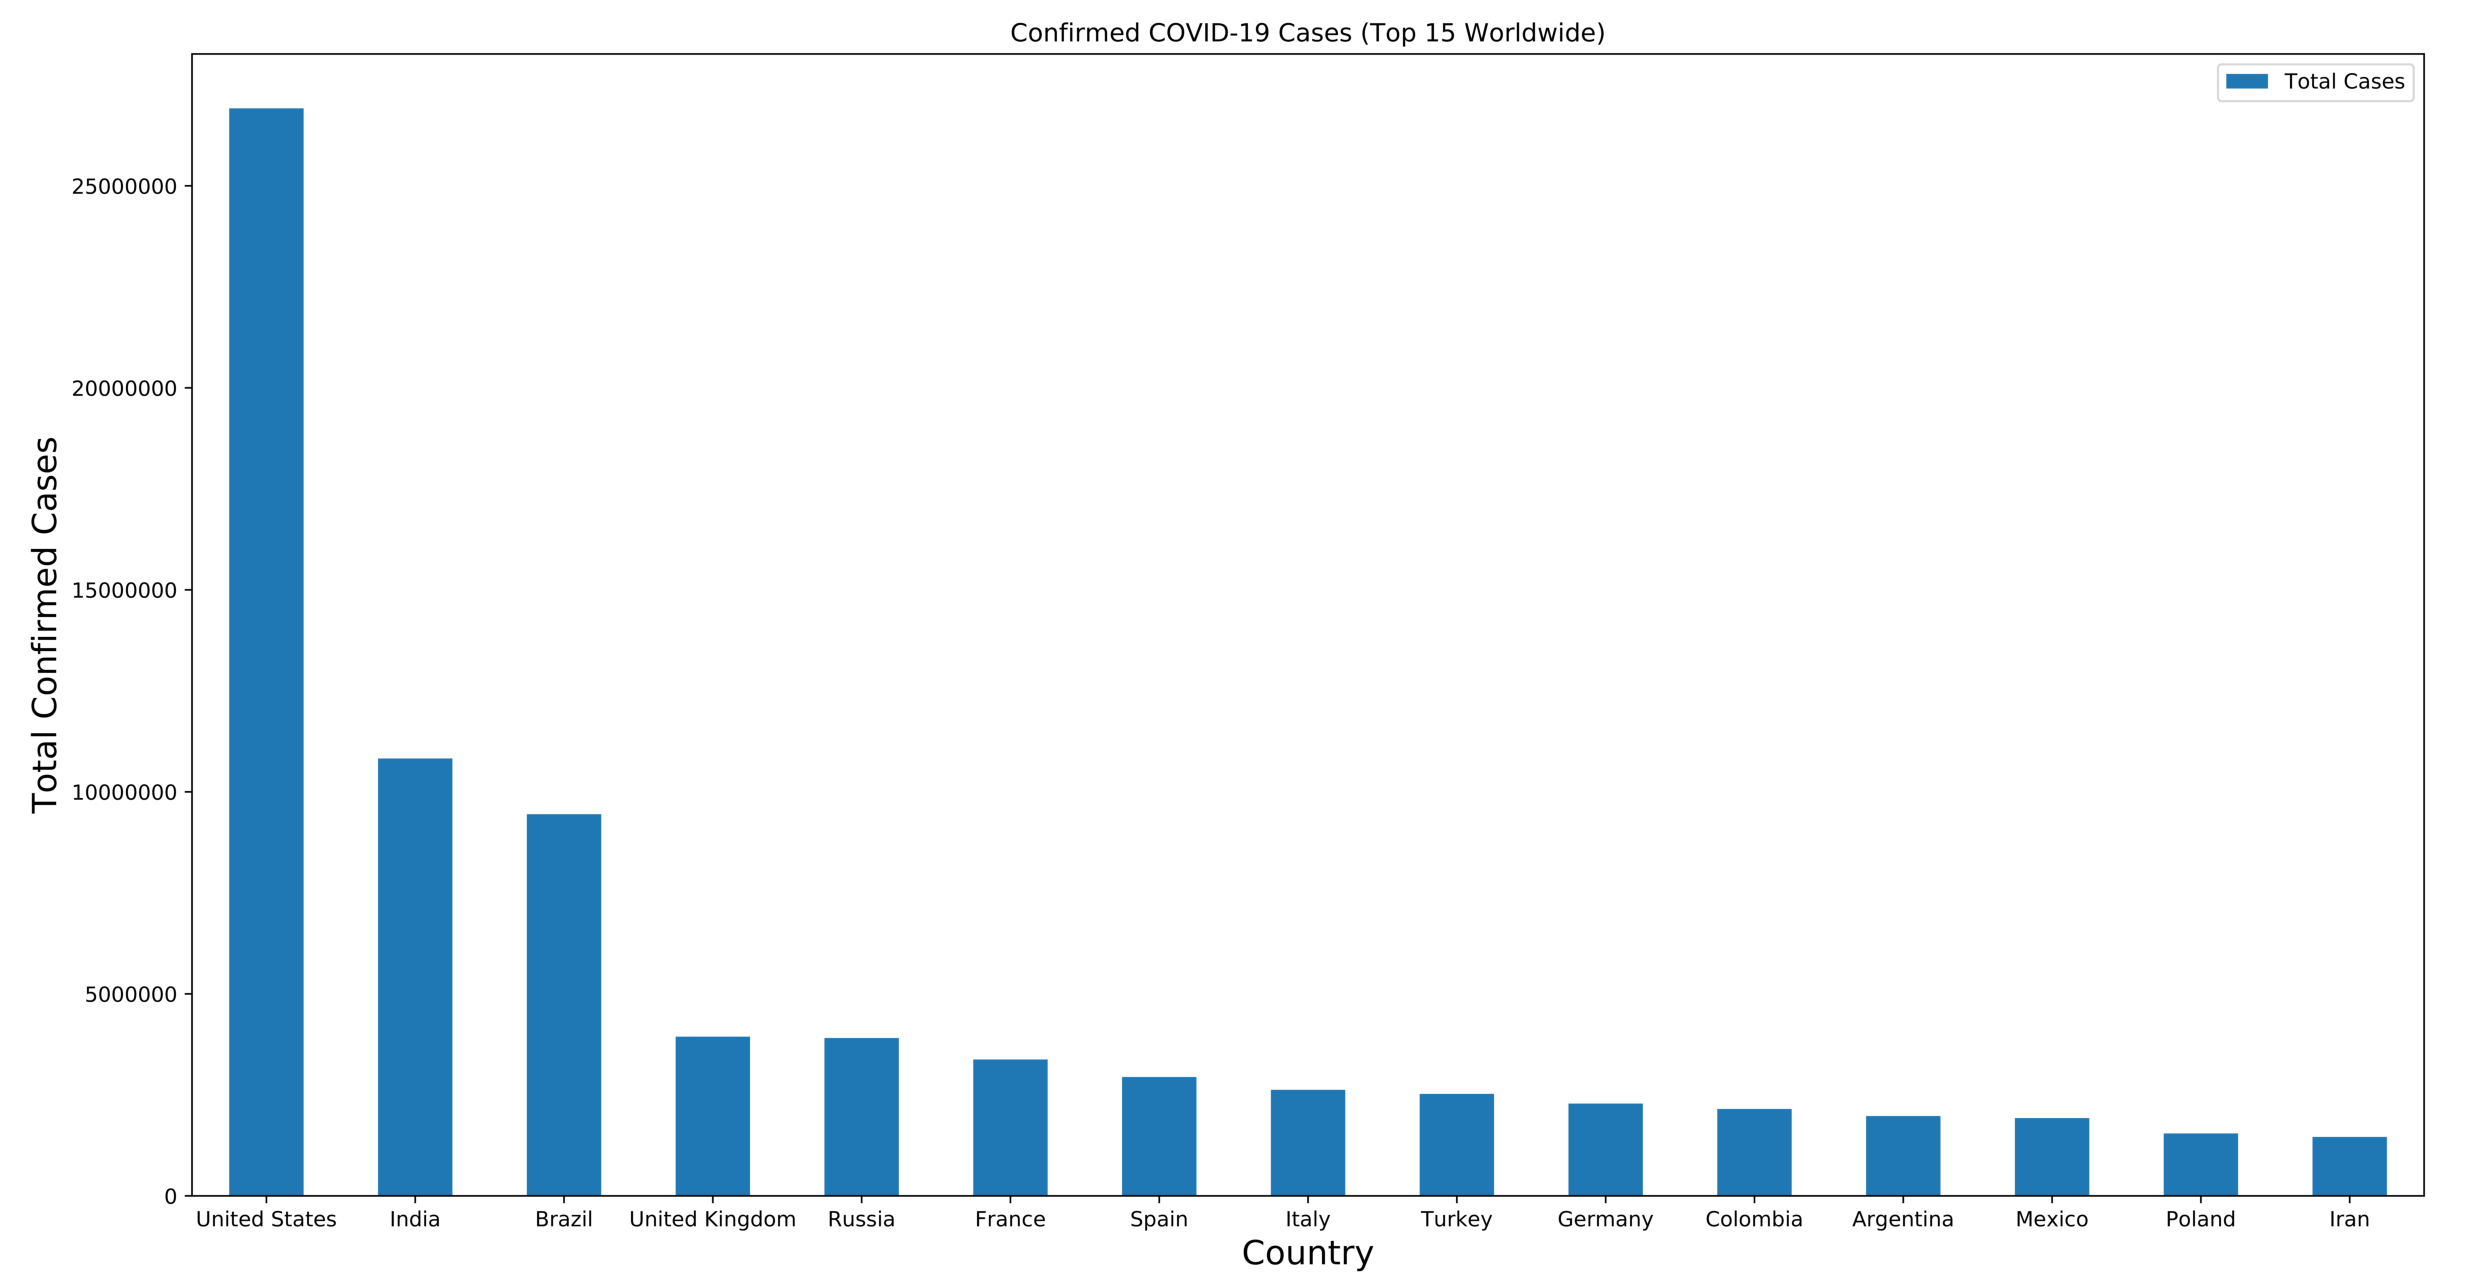
\includegraphics[scale=0.32]{img/total-cases.pdf}
    \end{center}
    \vspace{-0.3cm}
    \caption{Top 15 Countries Confirmed COVID-19 Cases}
\end{figure}
\noindent
Is this really the right choice? Does this ranking tells us anything meaningful
about the current undergoing pandemic situation? From what we can observe in
figure 1, clearly United States has higher confirmed COVID-19 cases than
countries such as Spain or Italy. Taking into account that the US is a much
bigger country, we can agree that this results do not imply that the US is more
affected than Spain, Italy or Germany. We can therefore think of a fairer
comparison independent of the country size: the number of infections needs to be
normalized to the population of each country. This provides a more coherent view
of the countries most affected by COVID-19:
\begin{figure}[H]
    \begin{center}
        \hspace*{-0.2cm}
        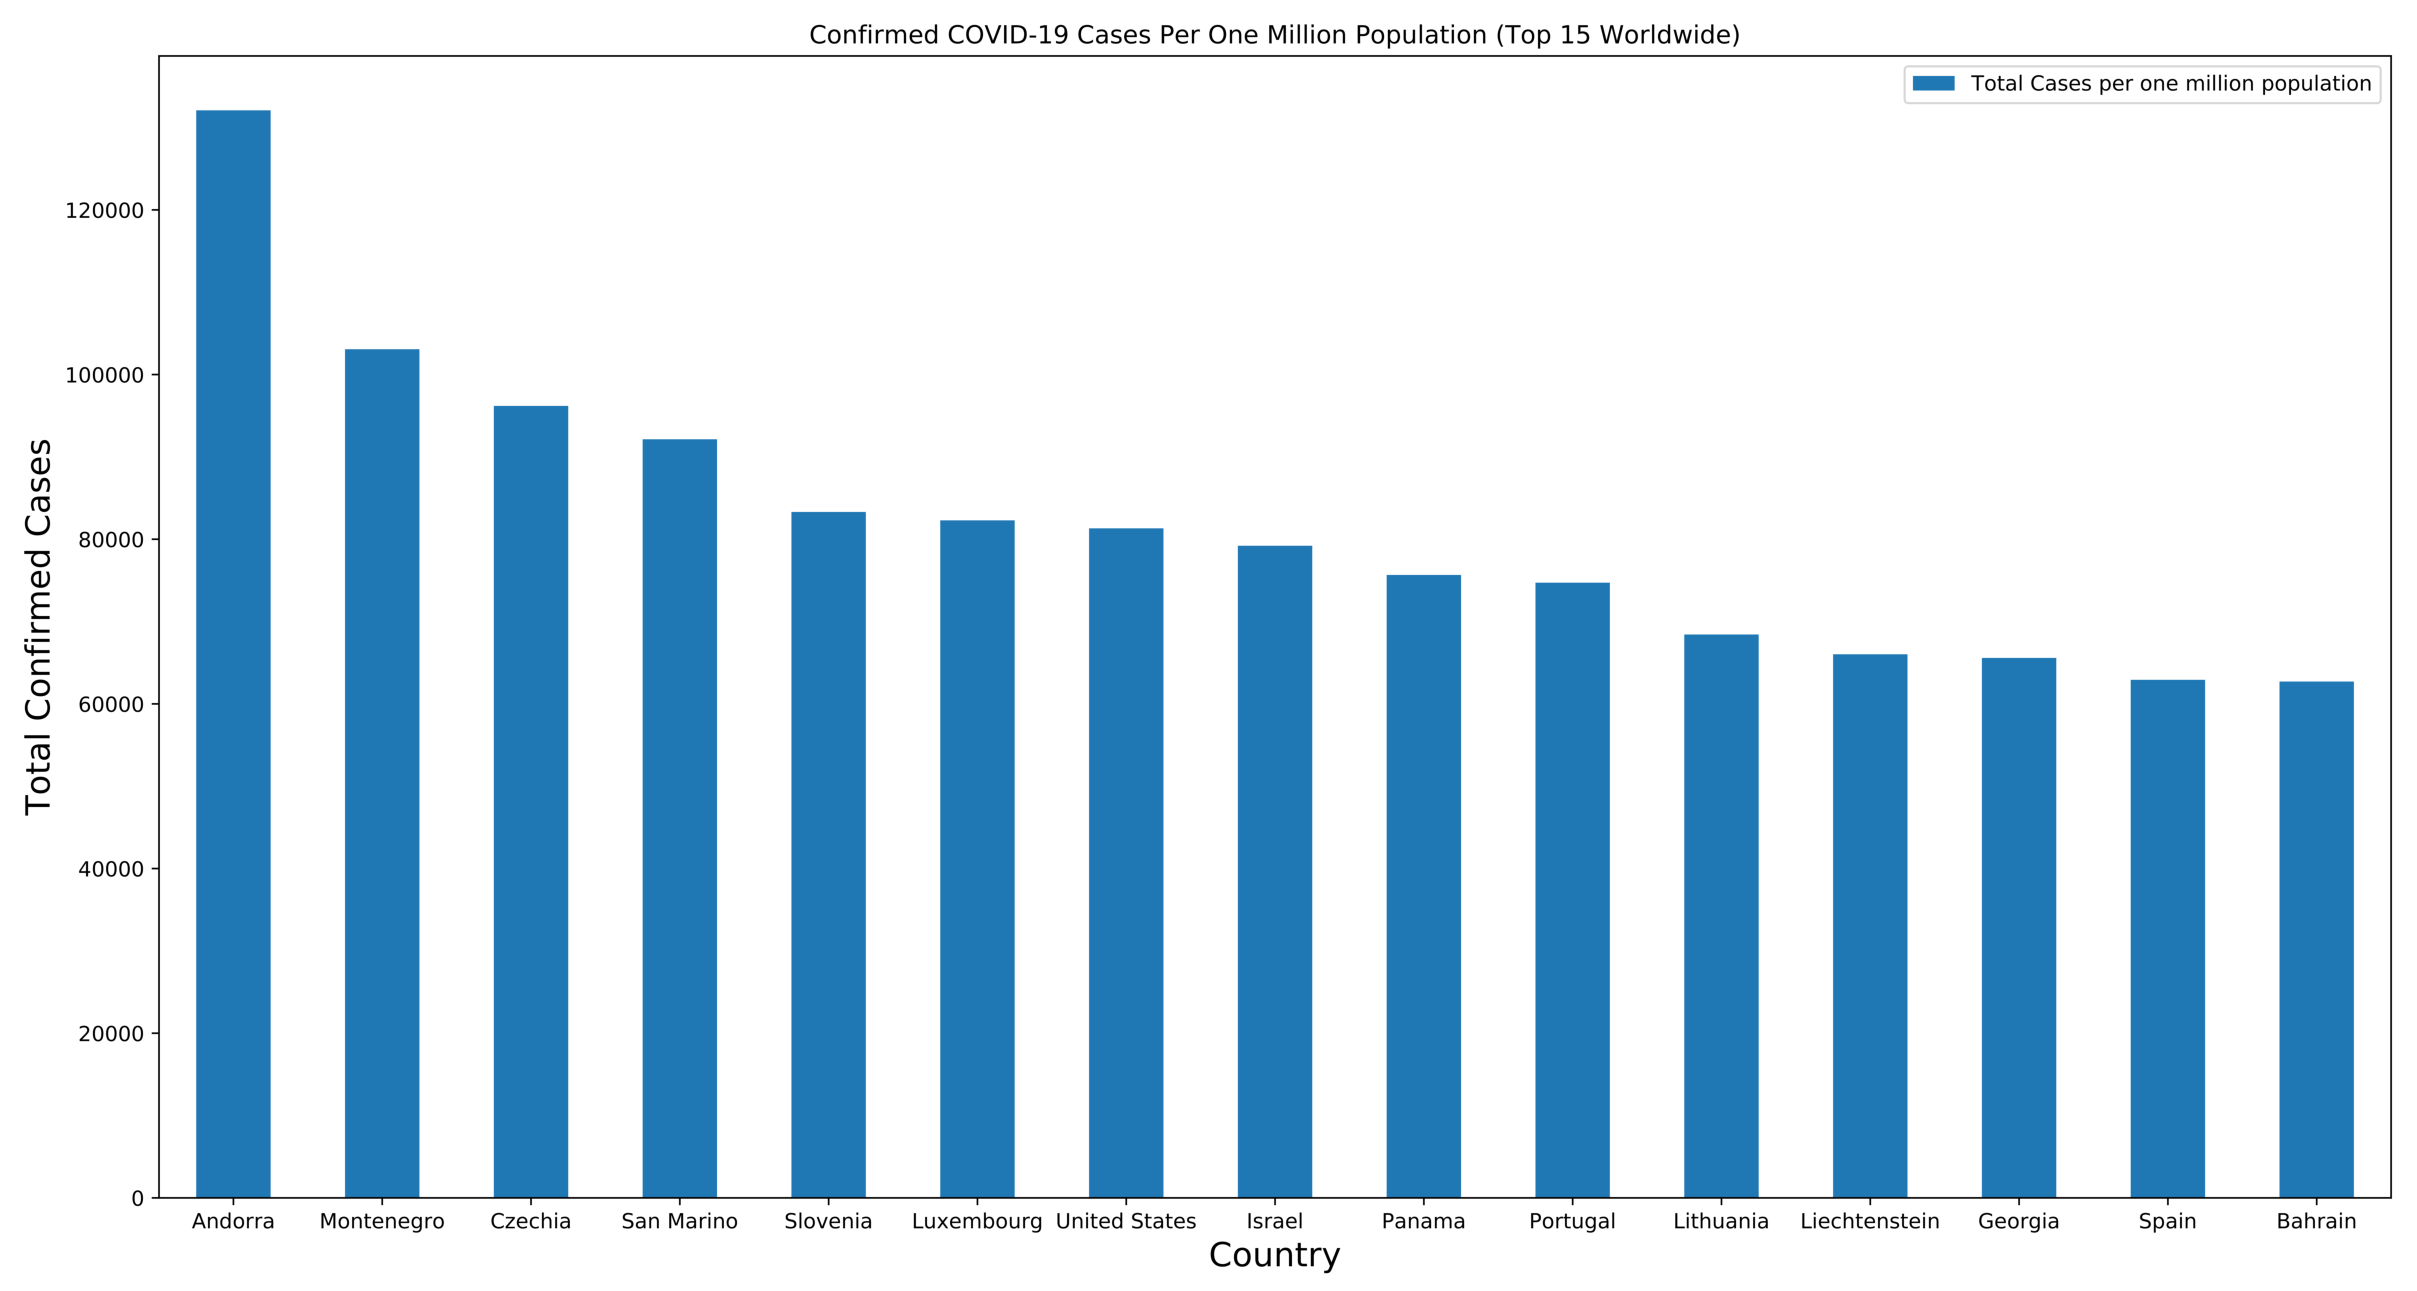
\includegraphics[scale=0.32]{img/total-cases-per-million.pdf}
    \end{center}
    \vspace{-0.3cm}
    \caption{Top 15 Countries Confirmed COVID-19 Cases Per One Million Population}
\end{figure}
\noindent
However it is not yet good enough: countries have different testing policies and
a more intensive COVID-19 testing rate gives more confirmed cases while no
testing at all would imply zero cases. We can all agree upon the fact that zero
cases with no testing at all does not really mean that a given country is not
affected by the pandemic. We therefore need a quantity unrelated to the rate of
testing.\\
This quantity is the number of deaths: this value is unbiased by the testing
rate. We will use the normalized number of daily deaths for comparing
countries.\\
\\
Before moving on, it is important to clarify that when we deal with COVID-19
deaths we refer to number of people who died in the COVID-19 time period
(starting from January 2020 till today). It is important to point out that
on the death certificate of these individuals there might be no reference at
all to the COVID-19 pandemic. This is because, as a result of different
policies in different countries worldwide, it is hard to obtain reliable
datasets with daily deaths that differentiate between those labeled COVID-19
and those completely related to other causes. Additionally, sometimes there is
no certainty about whether COVID-19 did or did not play a role in the death of
an individual.\\
\\
While the previous results were obtained using the original COVID-19 historical
dataset\cite{ourworldindata}, \textbf{this time some preprocessing and
resampling is needed}:
\begin{itemize}
    \item the daily values for some of the dates in the original dataset are missing:
    \begin{itemize}
        \item countries with too many missing values (more than $150$ days) were
        removed since no interpolation technique can really be effective in such
        cases;
        \item where few missing values were present for the initial months of
        the pandemic, these were replaced using the constant value $0$;
        \item missing and negative values in the middle of the time series were
        replaced using the moving window average;
    \end{itemize}
    \item plotting the data with daily granularity results in a time series plot
    which is not smooth and hard to read; the data was therefore resampled with
    weekly granularity;
\end{itemize}
To impute the missing values, i.e., to infer them from the known part of the
data, an univariate imputation algorithm was used: imputes values in the
i-th feature dimension using only non-missing values in that feature dimension.
To this end, the \texttt{SimpleImputer} class from the \texttt{scikit-learn}
Python package and the \texttt{rolling} method from the
\texttt{pandas.DataFrame} package were used.\\
\\
This is the resulting time series plot for some of the countries:
\begin{figure}[H]
    \begin{center}
        \hspace*{-0.3cm}
        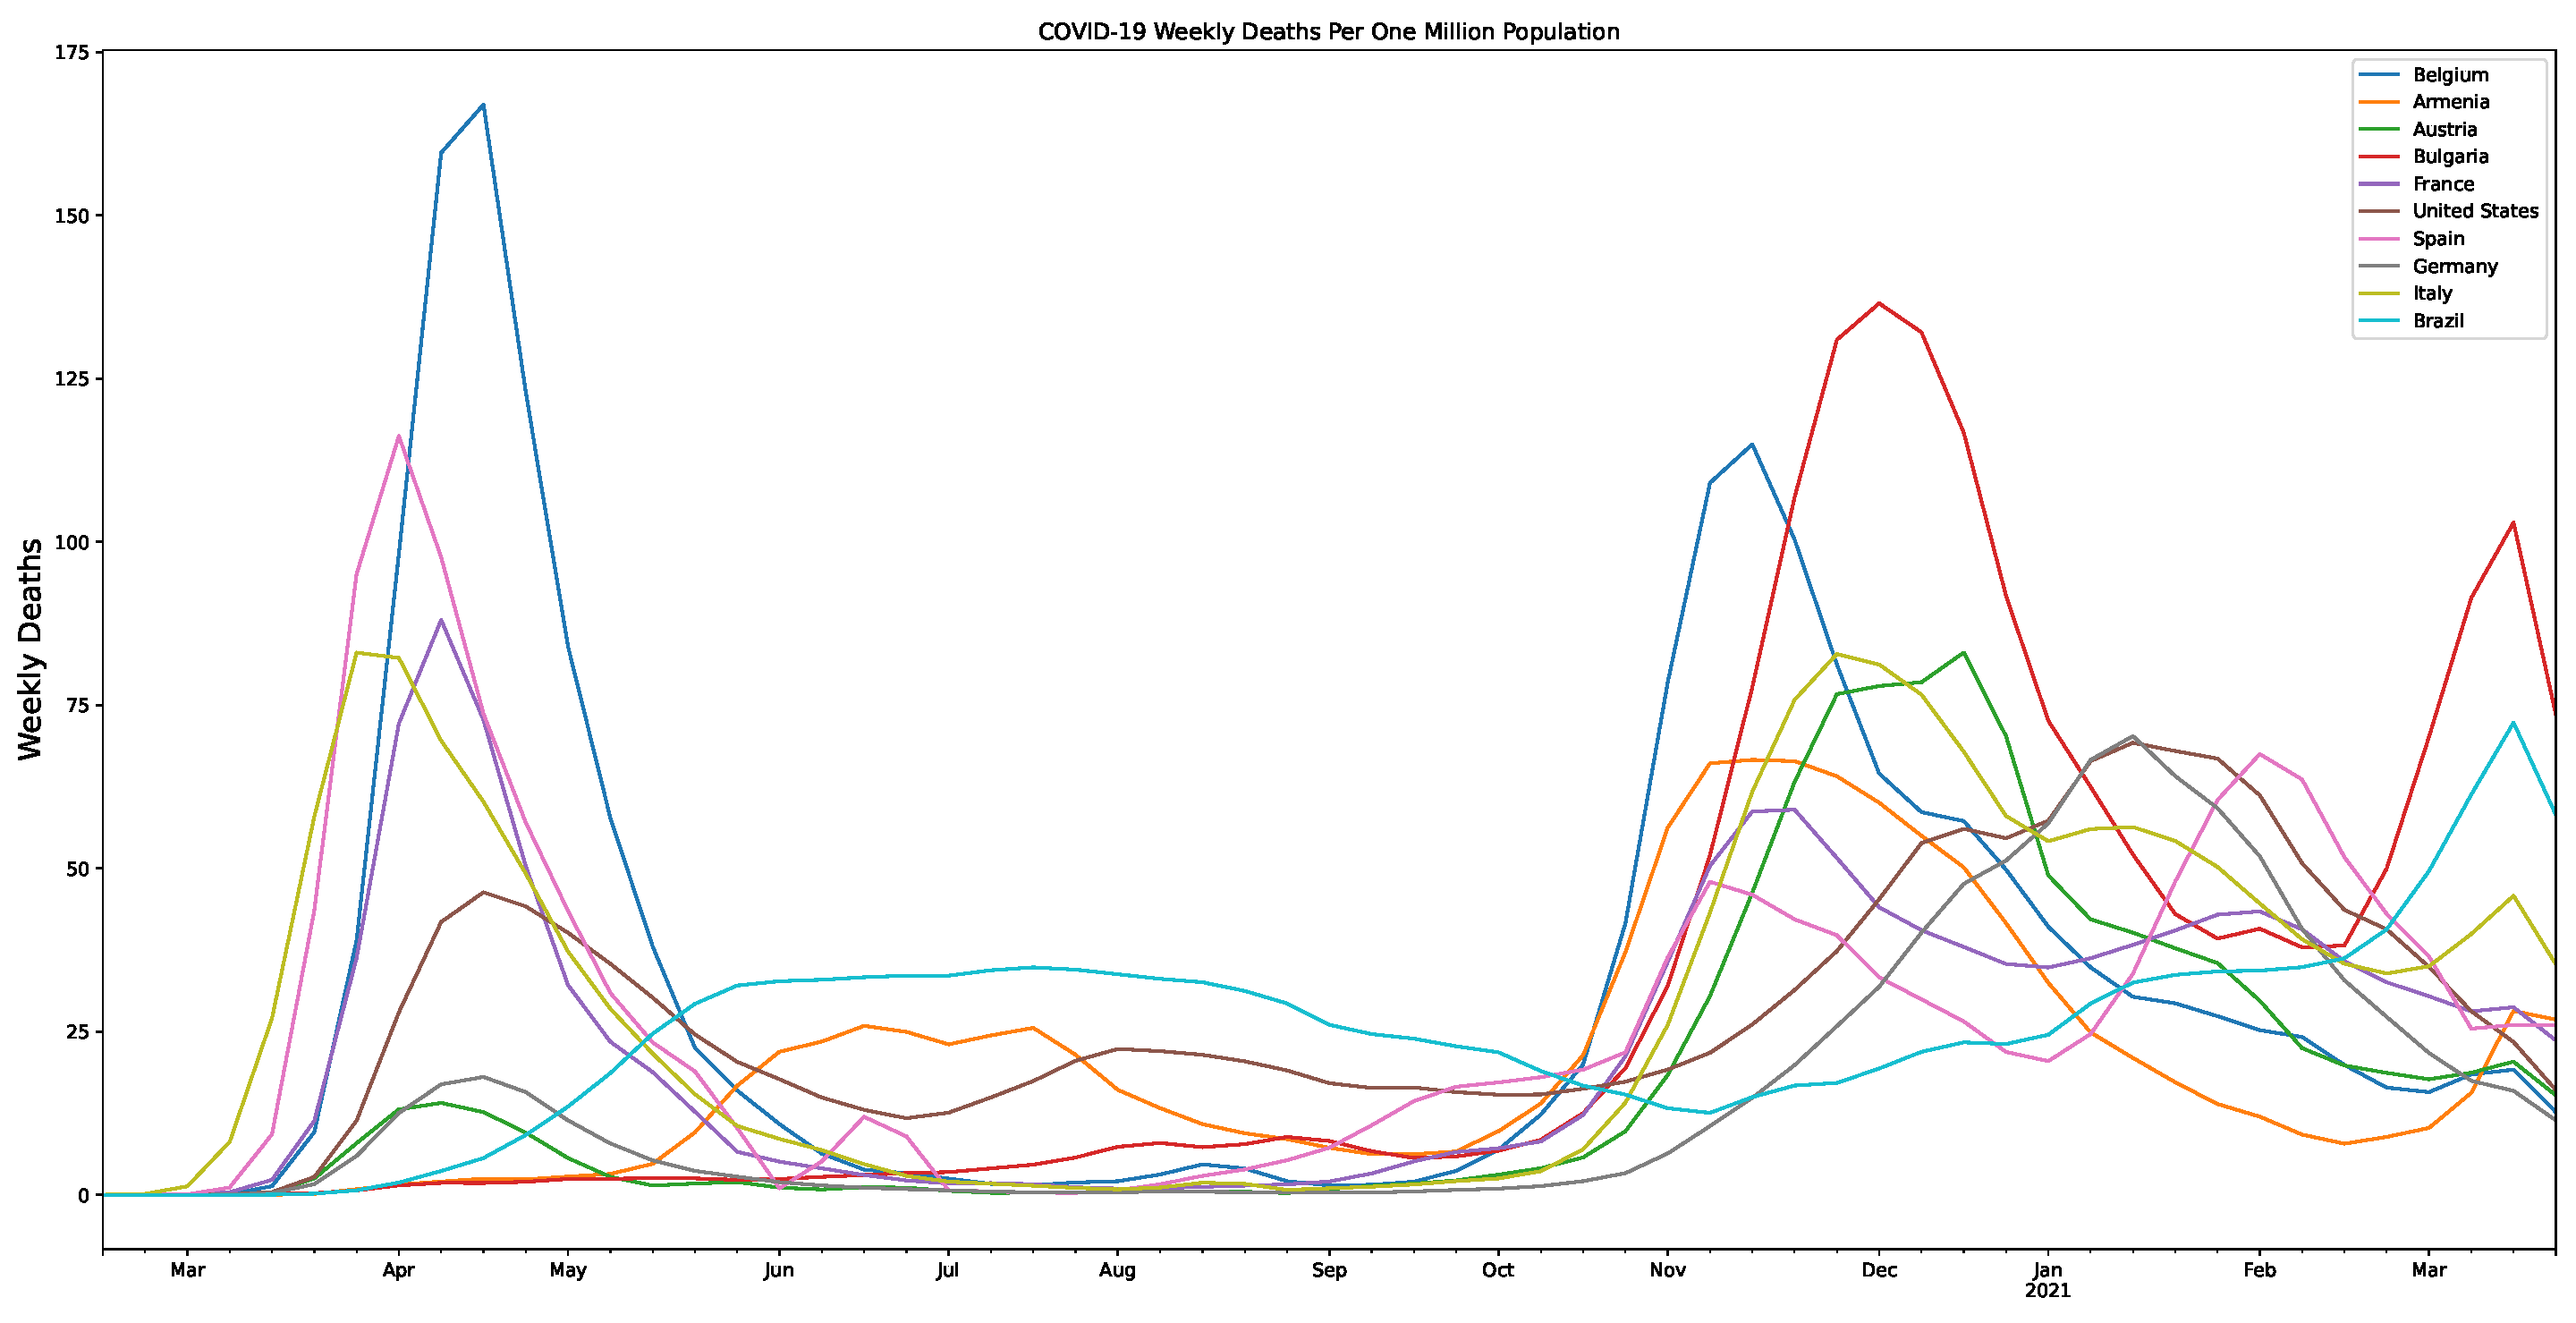
\includegraphics[scale=0.325]{img/weekly-deaths-per-million.pdf}
    \end{center}
    \vspace{-0.3cm}
    \caption{COVID-19 Weekly Deaths Per One Million Population}
\end{figure}
\noindent
Daily deaths count appears to be a fair measure to compare how hard different
countries have been hit by the virus. In addition, observing the plot one can
immediately point out that
\begin{itemize}
    \item some countries suffered more the first wave, some others the second
    and some others the third wave; some countries suffered all of them;
    \item countries such as {\color{ts_italy}Italy} and
    {\color{ts_belgium}Belgium} were devastated by the first wave and reacted
    by completely shutting down social life; yet they did not do better with the
    second wave; finally, the vaccination campaign seems to have helped them
    control the pandemic (both in {\color{ts_italy}Italy} and
    in {\color{ts_belgium}Belgium} almost $50\%$ of the population has received
    the first vaccine dose);
    \item countries such as {\color{ts_austria}Austria} and
    {\color{ts_germany}Germany} have not been hit hard by the first COVID-19
    wave; these states reacted fast and slowed down social life right at the
    beginning; as a result, the number of deaths went back to almost zero; yet
    they suffered from the second wave and got the situation under control using
    vaccines;
    \item countries such as {\color{ts_unitedstates}United States} and
    {\color{cyan}Brazil} had a daily death toll with an almost constant
    trend during the first and second waves; while the situation has drastically
    improved in the {\color{ts_unitedstates}United States} thanks to the
    vaccines ($50\%$ of the population has received
    the first vaccine dose), in {\color{cyan}Brazil} the number of daily deaths
    are increasing ($16\%$ of the population has received the first vaccine
    dose);
\end{itemize}
If we extend the same reasoning to all the countries, figure 4 shows the weekly
deaths per one million population for 200 countries, from Afghanistan to
Zimbabwe. It is humanly impossible to extract any useful information from such a
plot. \textbf{However, in this mess, how many different characteristic curves
can we find?}
\begin{figure}[H]
    \begin{center}
        \hspace*{-0.3cm}
        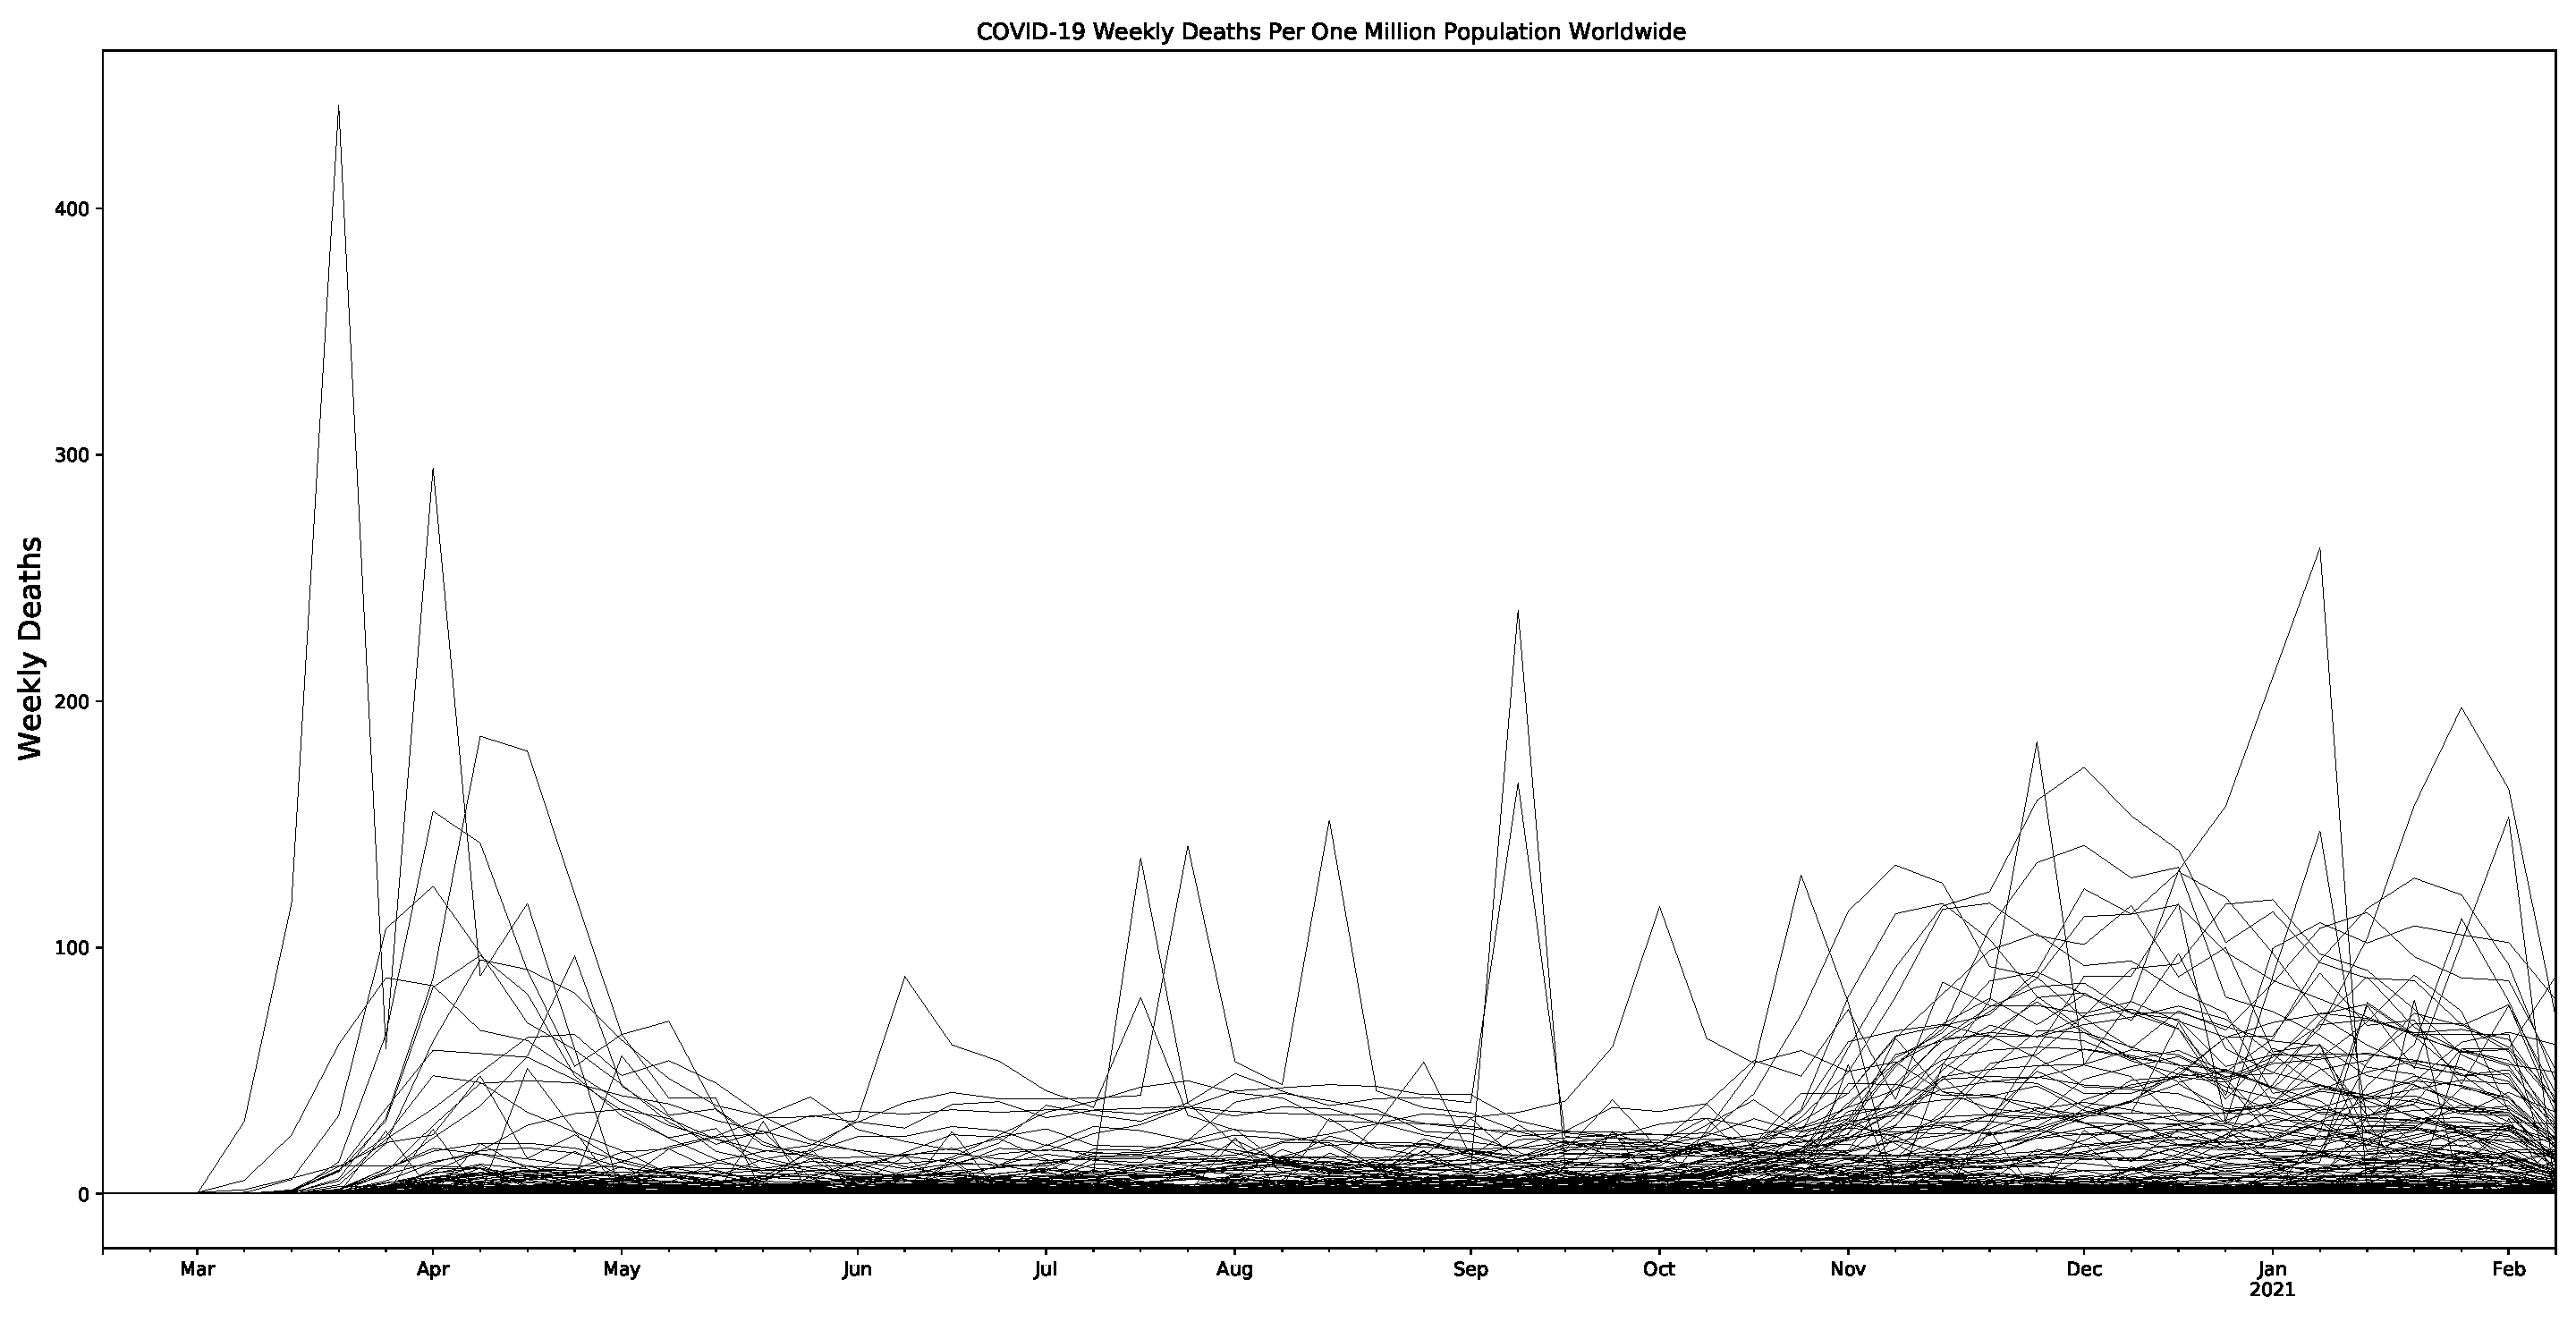
\includegraphics[scale=0.32]{img/weekly-deaths-worldwide.pdf}
    \end{center}
    \vspace{-0.3cm}
    \caption{COVID-19 Weekly Deaths Per One Million Population Worldwide}
\end{figure}
\noindent
To clean the mess, find patterns and extract the required knowledge, a
clustering algorithm was used. This unsupervised learning technique groups
similar data curves together.
\subsubsection{Clustering time series data}
When taking into account time series clustering algorithm, there have been
several measures applied. For example there is probability-based distance, that
takes into account the seasonality of data, Hausdorff distance defined as "the
maximum of the distances from a point in any of the sets to the nearest point in
the other set" (Rote (1991)) or Hidden Markov model based distance used in
modelling complex time series (Zeng, Duan, and Wu (2010)). The most popular
however is the Euclidean distance and Dynamic Time Warping distance. It has been
proven that the Euclidean distance is the most efficient, but forces both time
series to be the same length. The DTW method is however known to be the most
accurate.\\
\\
\textbf{Euclidean vs. Dynamic Time Warping}\\
The main difference between both distances can be best understood graphically.
The picture below shows an example of matched points of two data vectors. They
were connected based on the minimal distance between points based on DTW (black)
and Euclidean (red) distance. It can be seen that with DTW the 11th blue point
matches 4 green points. When taking into account the Euclidean distance it can
be seen that the assigned points 9-to-9 and 10-to-10 are visibly further than
9-to-11 and 10-to-11. That can significantly impact the overall distance of
series between each other. The DTW takes into account the shape of both time
series much better. Dynamic Time warping is a method of calculating distance
that is more accurate than Euclidean distance. It has an advantage over
Euclidean if data points are shifted between each other and we want to look
rather at its shape.
\begin{figure}[H]
    \begin{center}
        \hspace*{-0.3cm}
        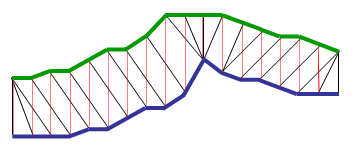
\includegraphics[scale=1.1]{img/euclidean-dtw.png}
    \end{center}
    \vspace{-0.2cm}
    \caption{Visual comparison of matched points based on DTW (black) and Euclidean (red) distance}
\end{figure}
\noindent
Additionally, the two time series do not have to be equal in length as required
by the Euclidean distance. The Euclidean distance takes pairs of data points and
compares them to each other. DTW calculates the smallest distance between all
points --- this enables a one-to-many match.\\
\\
Two K-means clustering models were built: one using the euclidean distance and
one using the DTW algorithm. To this end, \texttt{tslearn}, a Python package
that provides machine learning tools for the analysis of time series, was used.
This package builds on (and hence depends on) the \texttt{scikit-learn},
\texttt{numpy} and \texttt{scipy} libraries.\\
\\
First of all, the optimal number of clusters was evaluated using the mean
silhouette coefficient for all samples. The different silhouette values obtained
for the K-means Model are listed below:
\begin{itemize}
    \item $2$ Clusters silhouette:
    \begin{itemize}
        \item Euclidean distance: $0.606$ --- Dynamic Time Warping: $0.689$
    \end{itemize}
    \item $3$ Clusters silhouette:
    \begin{itemize}
        \item Euclidean distance: $0.585$ --- Dynamic Time Warping: $0.627$
    \end{itemize}
    \item $4$ Clusters silhouette:
    \begin{itemize}
        \item Euclidean distance: $0.582$ --- Dynamic Time Warping: $0.620$
    \end{itemize}
    \item $5$ Clusters silhouette:
    \begin{itemize}
        \item Euclidean distance: $0.597$ --- Dynamic Time Warping: $0.619$
    \end{itemize}
\end{itemize}
The best value for the mean silhouette coefficient is obtained with only $2$
clusters. However, taking into account our knowledge of the phenomenon, we
expect to find $3$ clusters of countries:
\begin{enumerate}
    \item those hardly hit by both the first and the second wave, that
    implemented a proper vaccination campaign;
    \item those that have been hit by either the first or the second wave, that
    implemented a proper vaccination campaign;
    \item and those suffering COVID-19 deaths constantly, that have not the
    resources to implement an adequate vaccination campaign.
\end{enumerate}
Two K-means models with $3$ clusters were therefore evaluated: one trained using
the euclidean distance and the other using the dynamic time warping algorithm.
\begin{figure}[H]
    \begin{center}
        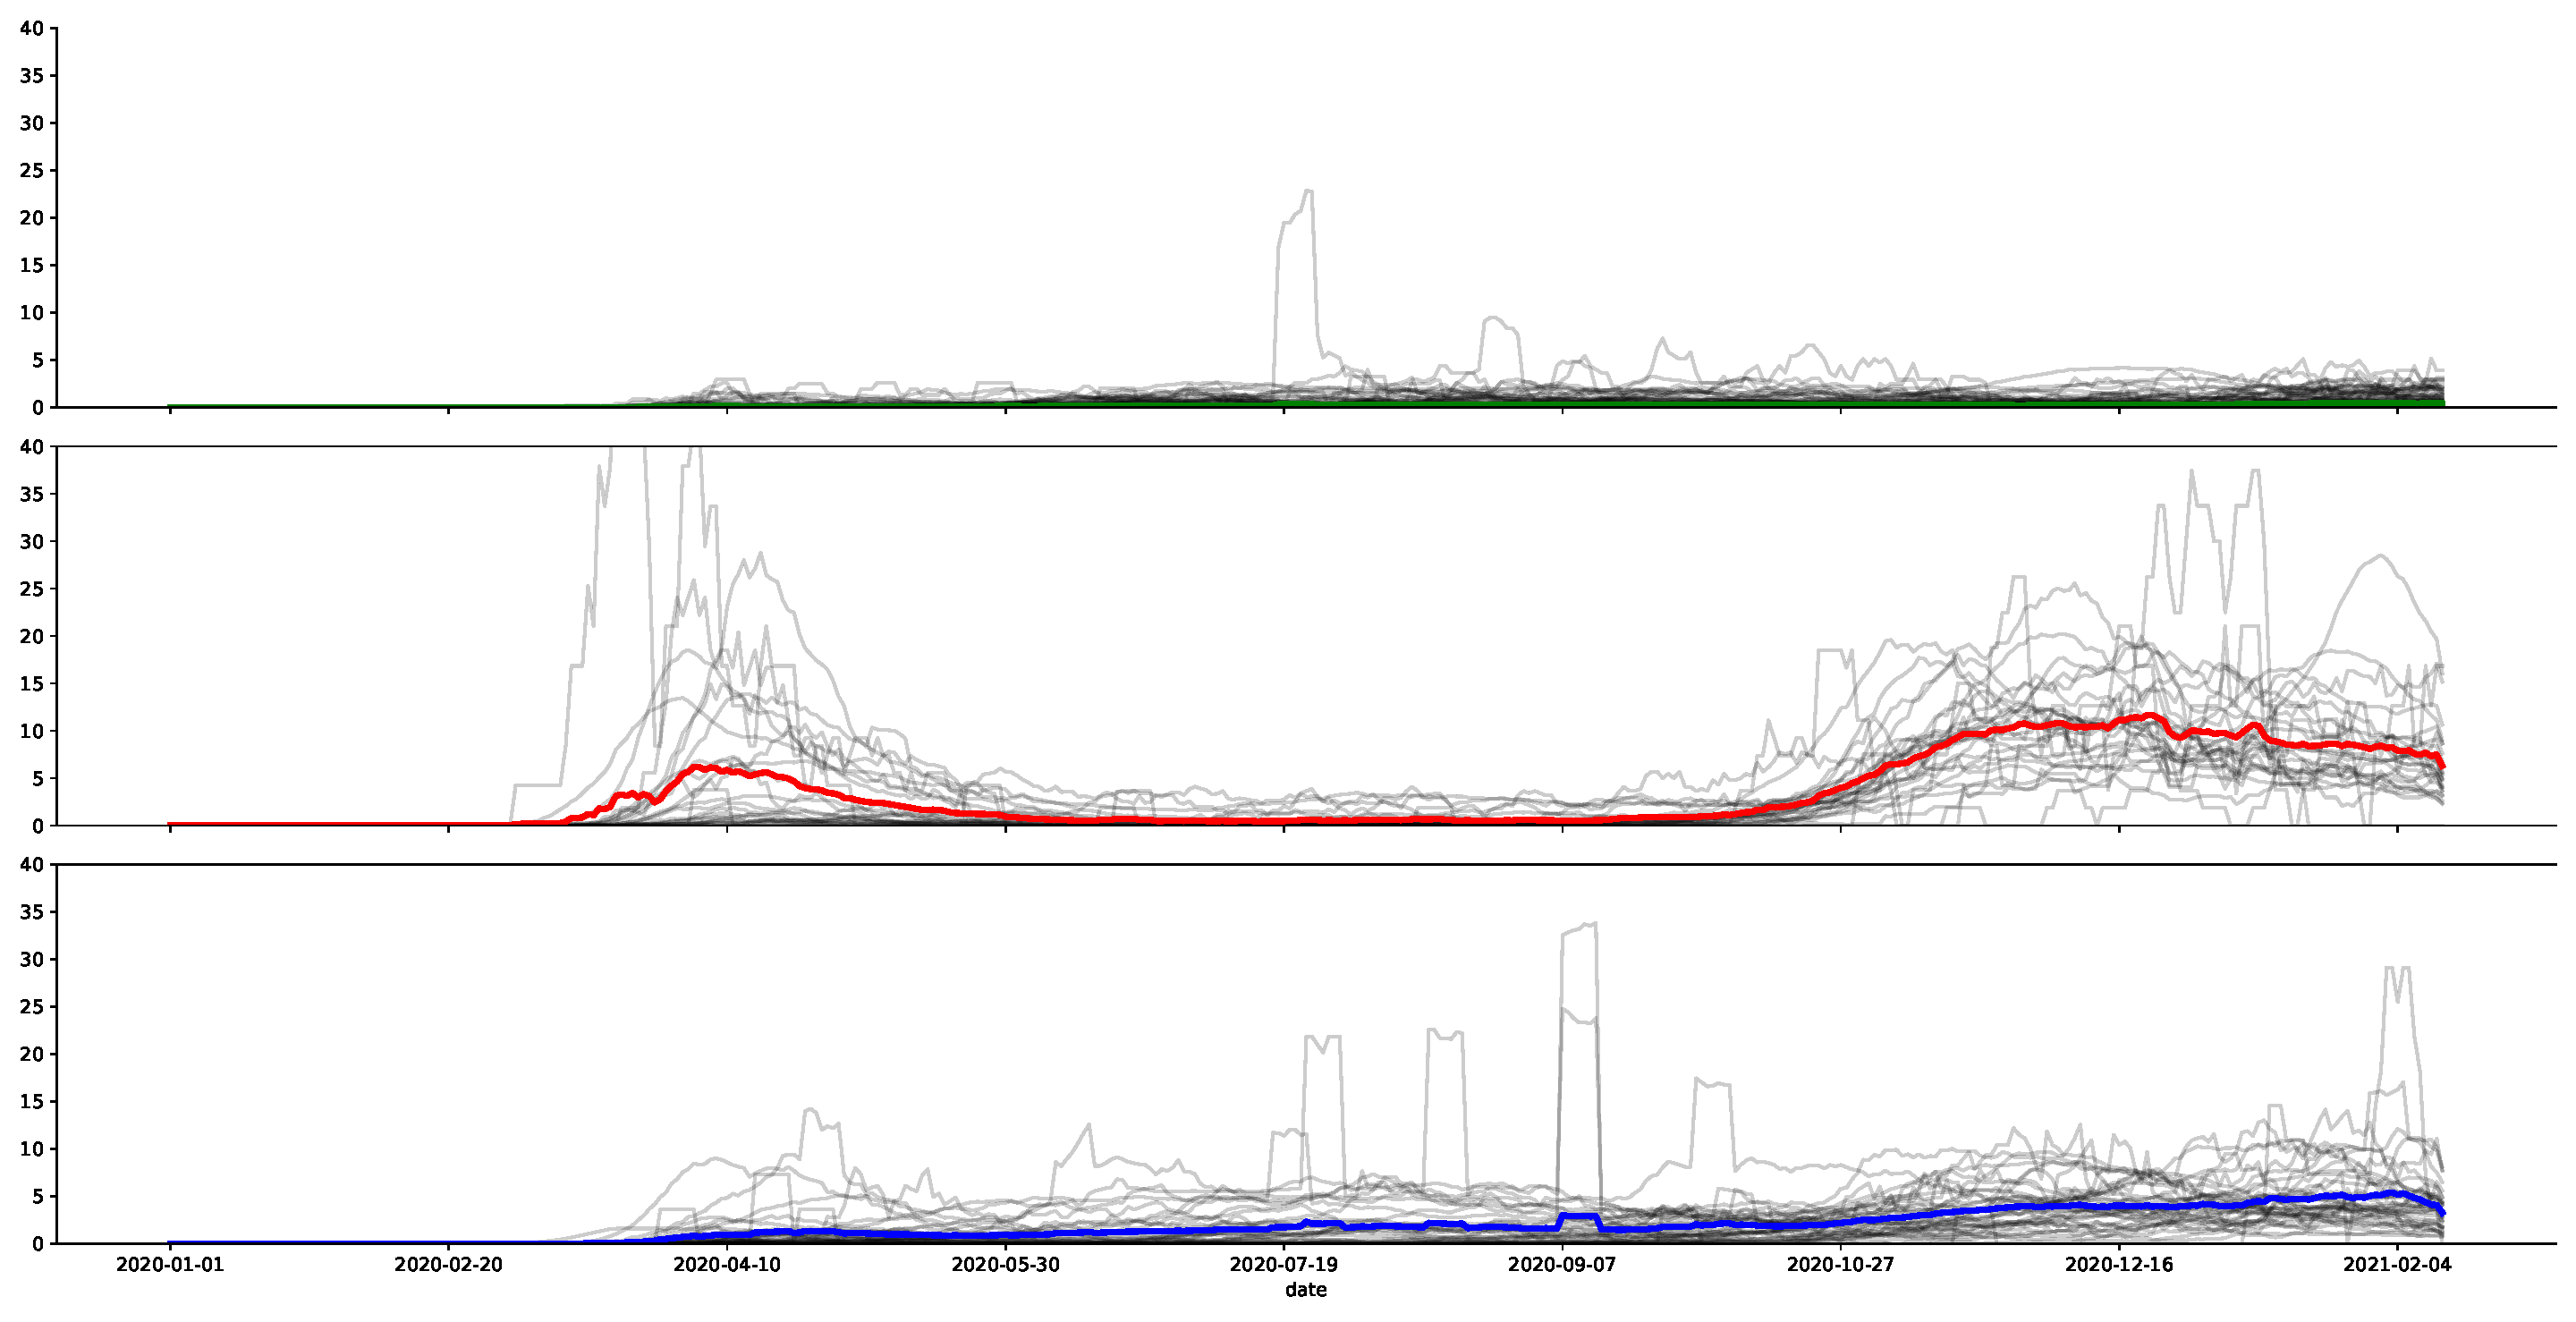
\includegraphics[scale=0.32]{img/daily-deaths-euclidean-clusters.pdf}
    \end{center}
    \vspace{-0.3cm}
    \caption{Time series K-means Clustering Model using Euclidean distance}
\end{figure}
\noindent
Figure 6 shows the clusters obtained by applying the K-means Clustering
algorithm provided by the \texttt{TimeSeriesKMeans} class of the
\texttt{tslearn} Python package. In this model, the metric chosen to be used for
both cluster assignment and barycenter computation is the euclidean distance:
\begin{itemize}
    \item the {\color{ForestGreen}green cluster} groups $167$ countries with
    a low number of daily deaths (close to zero);
    \item the {\color{blue}blue cluster} groups $11$ countries which suffered
    either the first or the second SARS-CoV-2 wave;
    \item the {\color{red}red cluster} groups $44$ countries with a huge number
    of daily deaths, that managed to get the situation under control for a while
    after the first wave, but suffered for the second wave as well;
    \item mean silhouette coefficient for all samples: $0.58$.
\end{itemize}
The time series K-means clustering model using the Dynamic Time Warping
algorithm provides different clusters. As shown in figure 7,
\begin{itemize}
    \item the {\color{ForestGreen}green cluster} groups $140$ countries;
    \item the {\color{blue}blue cluster} groups $28$ countries;
    \item the {\color{red}red cluster} groups $54$ countries;
    \item mean silhouette coefficient for all samples: $0.62$.
\end{itemize}
We should keep in mind that the DTW algorithm is quite CPU-intensive: as a
matter of fact, with $50$ iterations, the same number used to obtain the model
with the euclidean distance, it takes almost $2$ minutes\footnote{Please take
this statistic as a very general one --- it is relative to an Intel Core
i7-7700K Processor (4 Cores 8 Threads @ 4.20 GHz).} to compute the clusters
shown in figure 7.
\begin{figure}[H]
    \begin{center}
        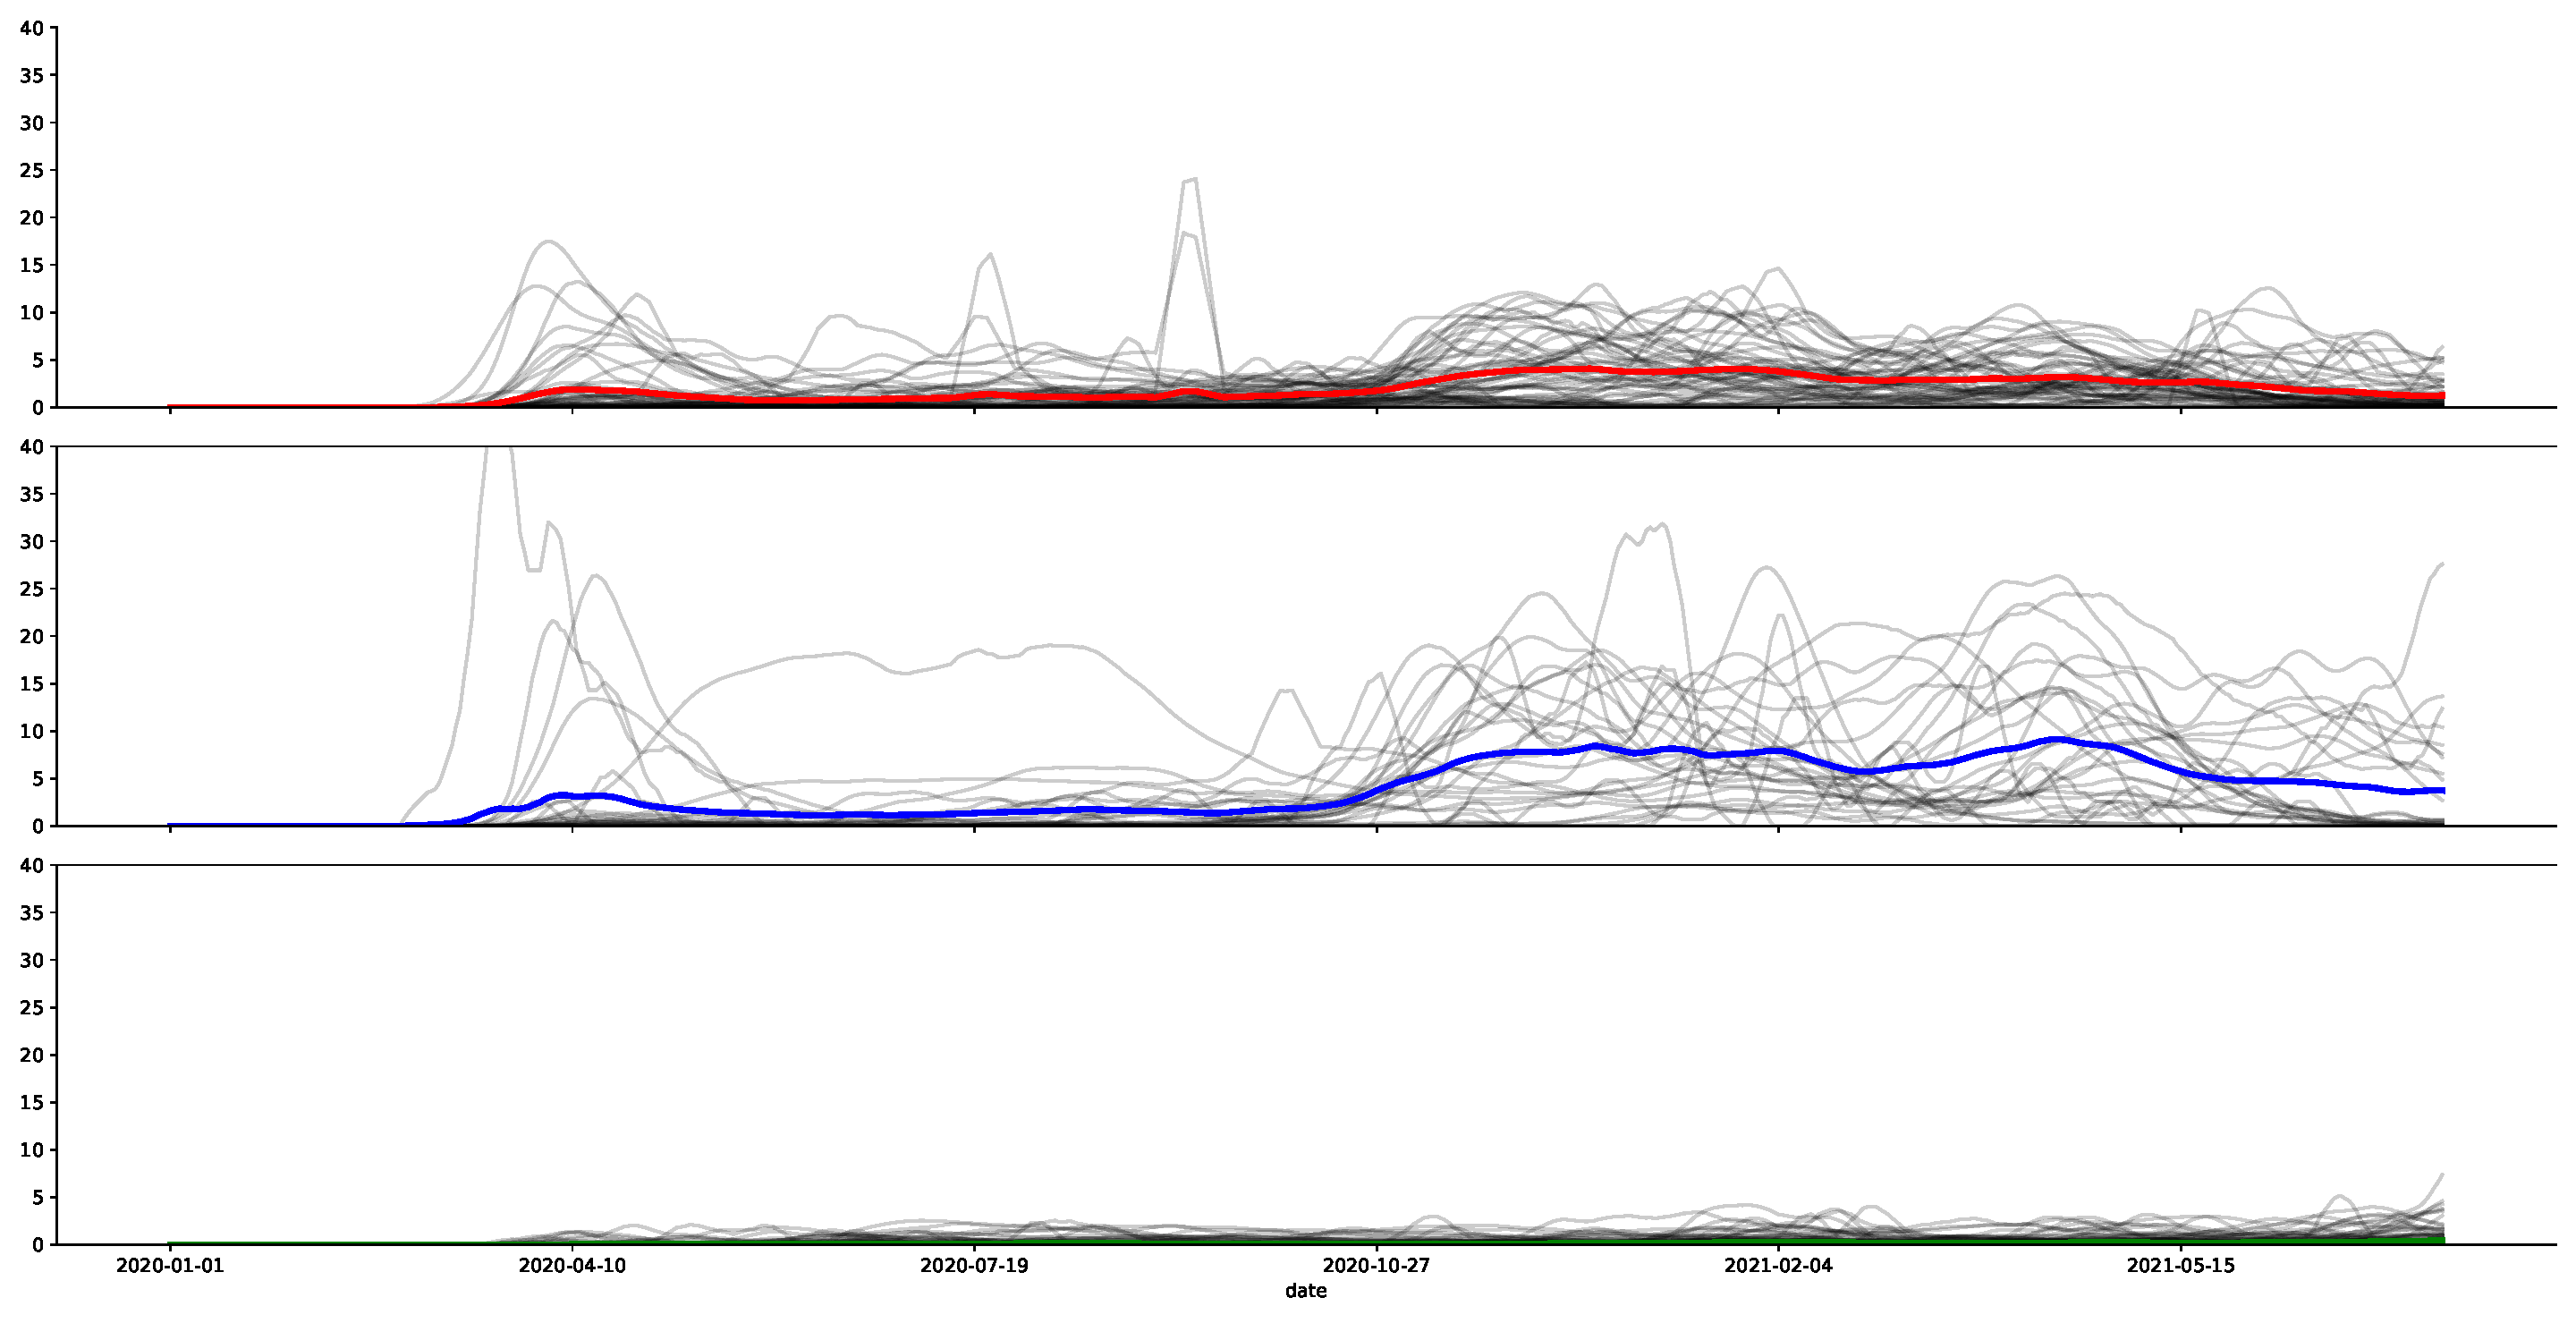
\includegraphics[scale=0.32]{img/daily-deaths-dtw-clusters.pdf}
    \end{center}
    \vspace{-0.3cm}
    \caption{Time series K-means Clustering Model using Dynamic Time Warping algorithm}
\end{figure}
\noindent
Simply looking at the characteristic curves of each of the clusters identified
in the two proposed models, it looks like that the DTW-based K-means clustering
performed a better grouping.\\
\\
Keeping in mind that
\begin{enumerate}
    \item the tools available in the \texttt{tslearn} Python package for working
    with time series clustering are quite limited;
    \item as a result the silhouette coefficient was used at the beginning in
    absence of other more robust clustering tendency statistical indicator;
    \item there is no real ground truth when dealing with clustering problems in
    general;
\end{enumerate}
to compare the two models, I represented the clusters obtained by the two models
on the world map. Surprisingly enough, as shown in figure 8 and in figure 9,
those groups form local clusters on the world map as well. The nature of the
phenomenon we are analyzing, the spread of the SARS-CoV-2 pandemic, tells us
that how well this local clusters are grouped in the world map, in terms of
neighboring countries can be used as a measure of how well the algorithm
performed:
\begin{figure}[H]
    \begin{center}
        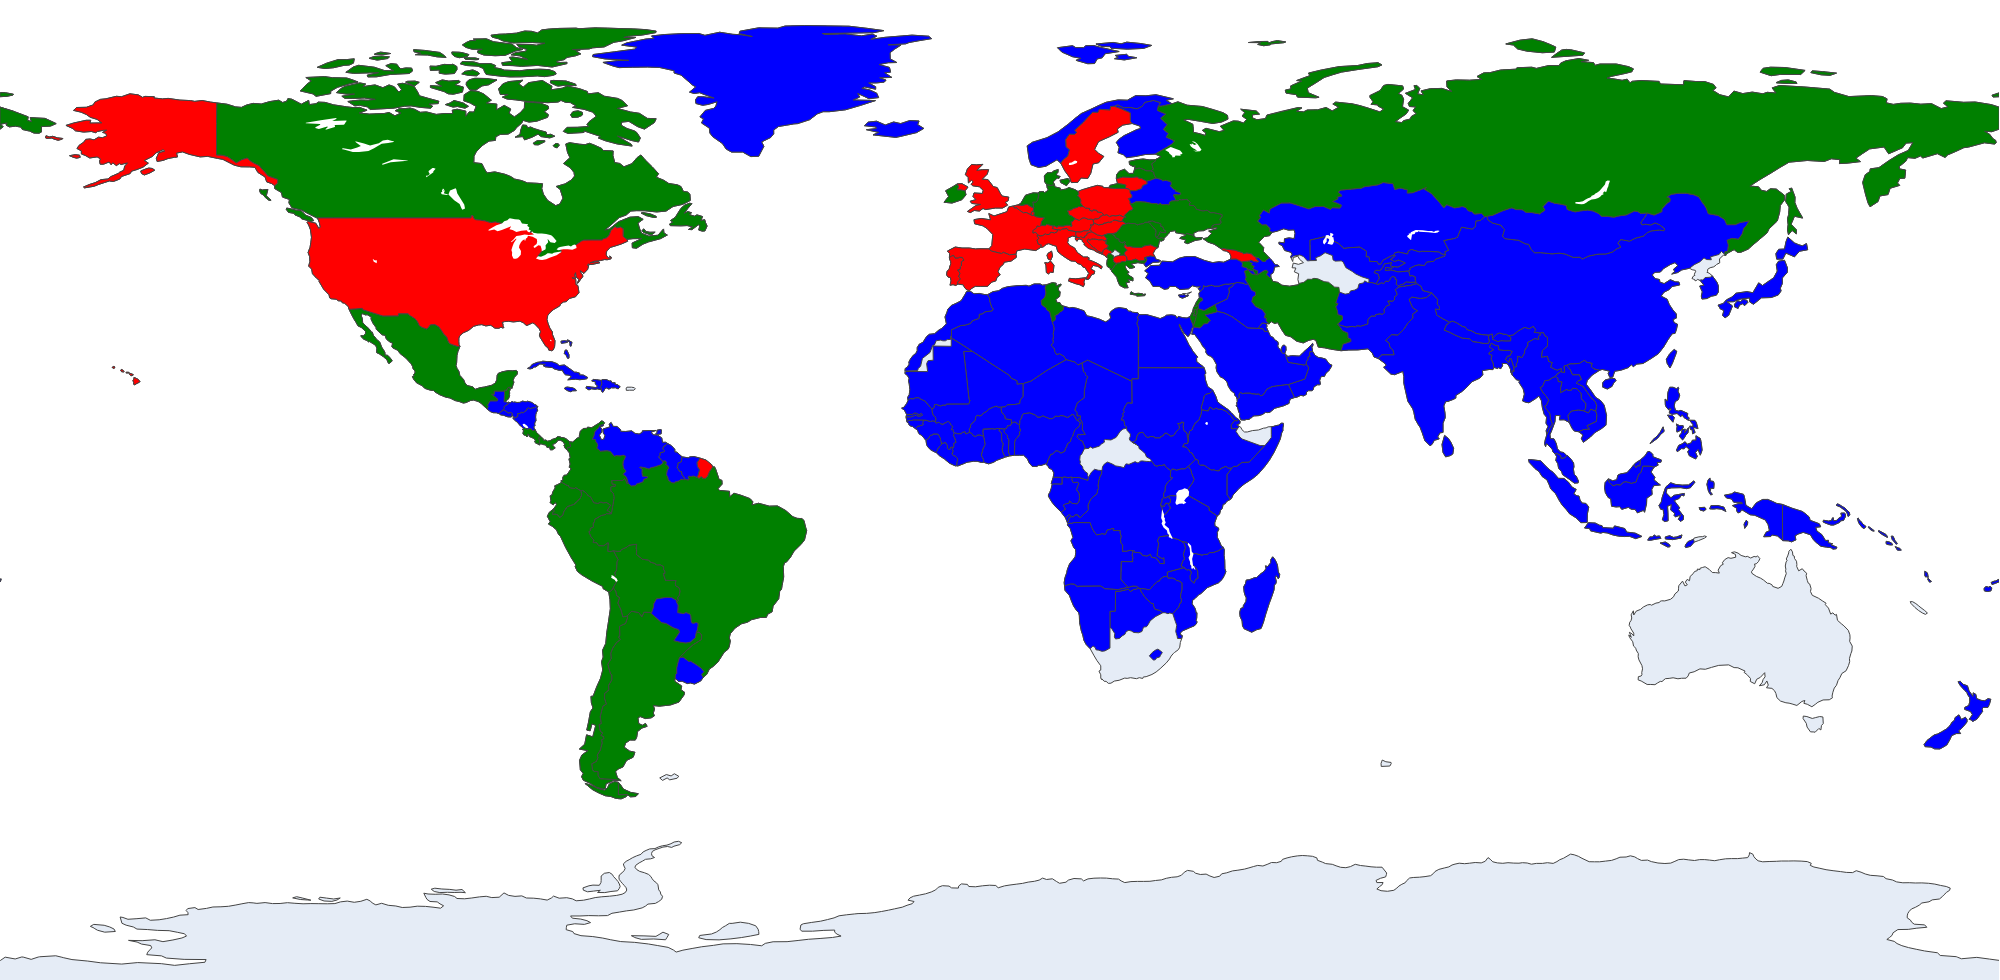
\includegraphics[scale=0.22]{img/euclidean-clusters-map.png}
    \end{center}
    \vspace{-0.2cm}
    \caption{K-means Clustering Model World Map (Euclidean Distance)}
\end{figure}
\noindent
Given the nature of the phenomenon under analysis, it is very hard to say which
is better. One important observation to be made is that changing from the
euclidean distance to the DTW algorithm, Canada moves from the
{\color{ForestGreen}green cluster} to the {\color{red}red cluster}. Also Russia
moved from the {\color{ForestGreen}green cluster} to the {\color{blue}blue
cluster}.
\begin{figure}[H]
    \begin{center}
        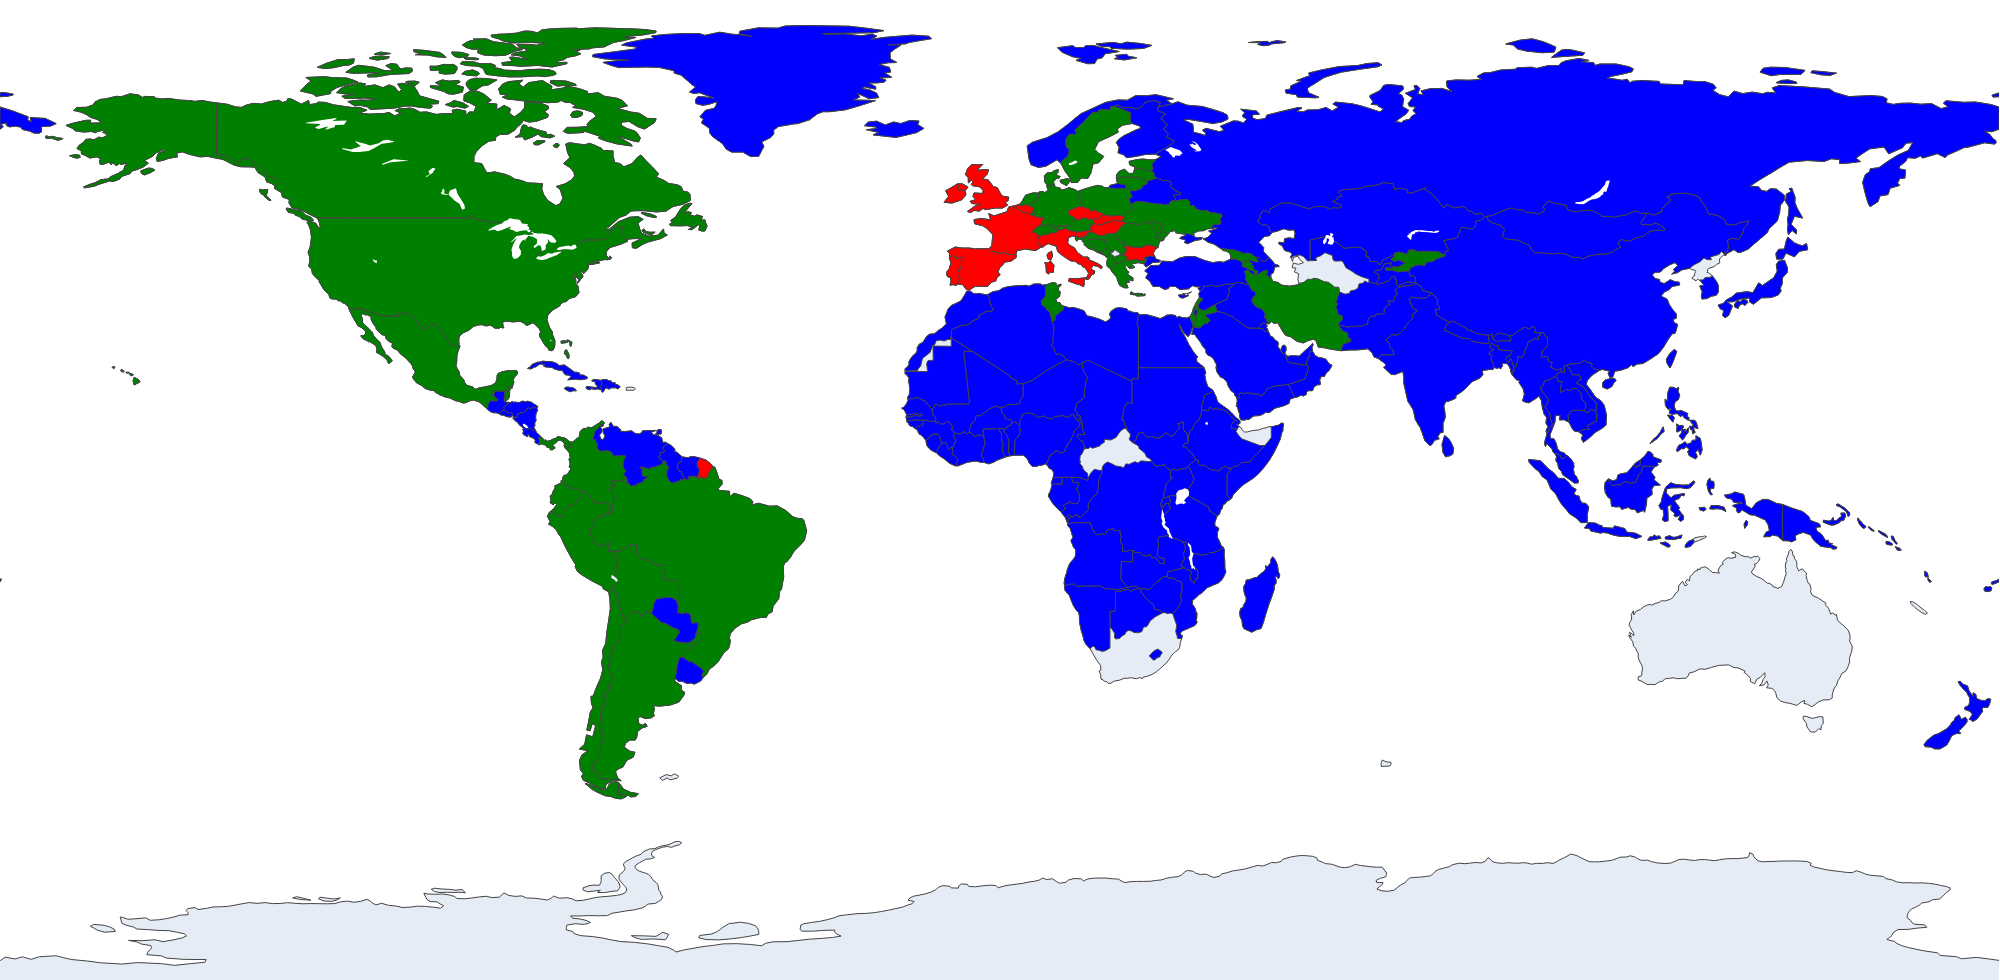
\includegraphics[scale=0.22]{img/dtw-clusters-map.png}
    \end{center}
    \vspace{-0.2cm}
    \caption{K-means Clustering Model World Map (DTW Algorithm)}
\end{figure}
\noindent
\begin{itemize}
    \item The {\color{ForestGreen}green cluster} (countries) corresponds to a
    two-wave profile, with the first peak at around Day $140$, and values
    reaching $7$ cases per $100,000$ of the population. The second wave started
    around Day $240$ and seems not to have peaked yet at Day $250$. These are
    also countries which started an adequate vaccination campaign in order to
    prevent a third wave: on average, almost $60\%$ of the population has
    received the second dose of the COVID-19 vaccine;
    \item The {\color{blue}blue cluster} groups countries which had a
    daily death toll with an almost constant trend during the first and second
    waves and did not succeed in running reactive vaccination campaign: on
    average, almost $20\%$ of the population has received the second dose of the
    COVID-19 vaccine;
    \item The {\color{red}red cluster} groups African and Middle East countries
    for which concern grows over third wave of infections. The number of deaths
    recorded for the past week has risen by more than $40\%$ compared with the
    previous week, according to the World Health Organization (WHO): on average,
    less than $10\%$ of the population has received the second dose of the
    COVID-19 vaccine.
\end{itemize}
Also, some \textbf{outliers} can be identified with reference to this map:
\begin{itemize}
    \item Lebanon, Oman, Nepal, Kyrgyzstan, Tunisia, Botswana and Namibia which
    are classified as {\color{ForestGreen}green countries} but should be part
    of the {\color{red}red counties}: this is highly related to the fact that
    the data provided by such countries might no be reliable;
    \item Israel which is the country with the one of the highest percentages
    of vaccinated citizens and is classified as a {\color{red}red country}.
\end{itemize}
In conclusion, I believe that it is not easy to model a complex phenomenon such
as the COVID-19 just by using $3$ clusters based on the count of weekly deaths
per one million population.\\
\\
We also have to take into account that the clustering results are also
influenced by vaccinations campaigns. Such campaigns (where actually active) are
affected by geopolitics as well: politics and international relations play a
major role.
\subsection{Personalized predictive models for symptomatic COVID-19 patients}
Currently, the world is facing a health and economic crisis due to the spread of
the virus SARS-CoV-2 which causes a disease referred to as COVID-19. By the end
of April 2020, the virus has spread to over $191$ million people worldwide and
has killed over $4,1$ million. During this pandemic, governments and hospitals
have struggled to allocate scarce resources, including tests, treatment in
intensive care units (ICUs) and ventilators.\\
\\
The rapid global spread of the virus SARS-CoV-2 has provoked a spike in demand
for hospital care. Hospital systems across the world have been over-extended,
including in Northern Italy, Ecuador, and New York City, and many other systems
face similar challenges. As a result, decisions on how to best allocate very
limited medical resources have come to the forefront. Specifically, under
consideration are decisions on who to test, who to admit into hospitals, who to
treat in an Intensive Care Unit (ICU), and who to support with a ventilator.
Given today's ability to gather, share, analyze and process data, personalized
predictive models based on demographics and information regarding prior
conditions can be used to
\begin{enumerate}
    \item help decision-makers allocate limited resources;
    \item advise individuals how to better protect themselves given their risk
    profile;
    \item using risk profiles to inform decisions on who should be tested (for
    the virus and/or antibodies) and at which frequency;
    \item providing more accurate estimates of who is more likely to be
    hospitalized and the type of care they may need;
    \item informing plans for staffing, resources, and prioritizing the level of
    care in extremely resource-constrained settings.
    \item to develop personalized models that predict the following events:
        \begin{enumerate}
            \item hospitalization;
            \item mortality;
            \item need for ICU
            \item need for a ventilator.
        \end{enumerate}
\end{enumerate}
Equally importantly, as societies adapt to the pandemic, predictive models can
\begin{enumerate}
    \item assess individual risk so that social distancing measures can
    transition from "blanket" to more targeted (e.g., deciding who can return to
    work, who is advised to stay at home, who should be tested, etc.);
    \item direct policy decisions on who should receive priority for
    vaccination, which will be critical as initial vaccine production may not
    suffice to vaccinate everybody.
\end{enumerate}
Using the FPGrowth (Frequent Pattern Growth) algorithm\footnote{The
\texttt{frequent\_patterns} module of the \texttt{mlxtend} Python package was
used to this end.} allowed to mine the association rules listed in the following
table ordered by support value:
\begin{center}
\hspace*{-1cm}
\begin{tabular}{ | c | c | c | c | c | c | c | }
    \rowcolor{gray!50}
    \hline
    Antecedents & Consequents & Support & Confidence & Lift & Kulczynski & IR\\
    \hline
    Pneumonia & COVID-19, Hospitalization & 0.116372 & 0.859268 & 4.797504 & 0.0 & 0.0\\
    \hline
    Pneumonia & COVID-19, Hospitalization & 0.116372 & 0.859268 & 4.797504 & 0.0 & 0.0\\
    \hline
\end{tabular}
\end{center}
%-------------------------------------------------------------------------------
% Section: Conclusion
%-------------------------------------------------------------------------------
\newpage
\section{Conclusion}

%-------------------------------------------------------------------------------
% Section: Software Architecture
%-------------------------------------------------------------------------------
\newpage
\section{Software Architecture}
The subsequent analysis results were implemented as functionalities of a small
Python3 software:
\begin{lstlisting}[language=bash,frame=single]
$ python3 main.py 
Welcome to the COVID-19 Toolbox.

Type help or ? to list commands.

> ?

Documented commands (type help <topic>):
========================================
exit                              plot_weekly_deaths_per_million
help                              print_historical_ds_info
personalized_predictive_models    print_preconditions_ds_info
plot_total_cases                  timeseries_clustering_dtw
plot_total_cases_per_million      timeseries_clustering_euclidean
plot_weekly_deaths_all_countries  update_historical_ds
\end{lstlisting}
The following is a brief description of each of the available commands:
\begin{itemize}
    \item \texttt{update\_historical\_ds}: updates COVID-19 historical dataset to
    the latest available version;
    \item \texttt{print\_historical\_ds\_info}: prints COVID-19 historical dataset
    info;
    \item \texttt{print\_preconditions\_ds\_info}: prints COVID-19 preconditions
    dataset info;
    \item \texttt{plot\_total\_cases}: plot COVID-19 total confirmed cases
    histogram of the TOP 15 countries;
    \item \texttt{plot\_total\_cases\_per\_million}: plot COVID-19 total confirmed
    cases per one million population histogram of the TOP 15 countries;
    \item \texttt{plot\_weekly\_deaths\_per\_million}: plot COVID-19 weekly deaths
    per one million population time series of random countries;
    \item \texttt{plot\_weekly\_deaths\_all\_countries}: plot COVID-19 weekly deaths
    per one million population time series of all countries;
    \item \texttt{timeseries\_clustering\_euclidean}: plot COVID-19 daily deaths
    per one million population time series euclidean-based K-means clusters;
    \item \texttt{timeseries\_clustering\_dtw}: plot COVID-19 daily deaths per one
    million population time series DTW-based K-means clusters;
    \item \texttt{personalized\_predictive\_models}: build personalized predictive
    models for symptomatic COVID-19 patients using medical preconditions;
    \item \texttt{exit}: exit COVID-19 Toolbox.
\end{itemize}
\subsection{Class Diagram}
\begin{figure}[H]
    \begin{center}
        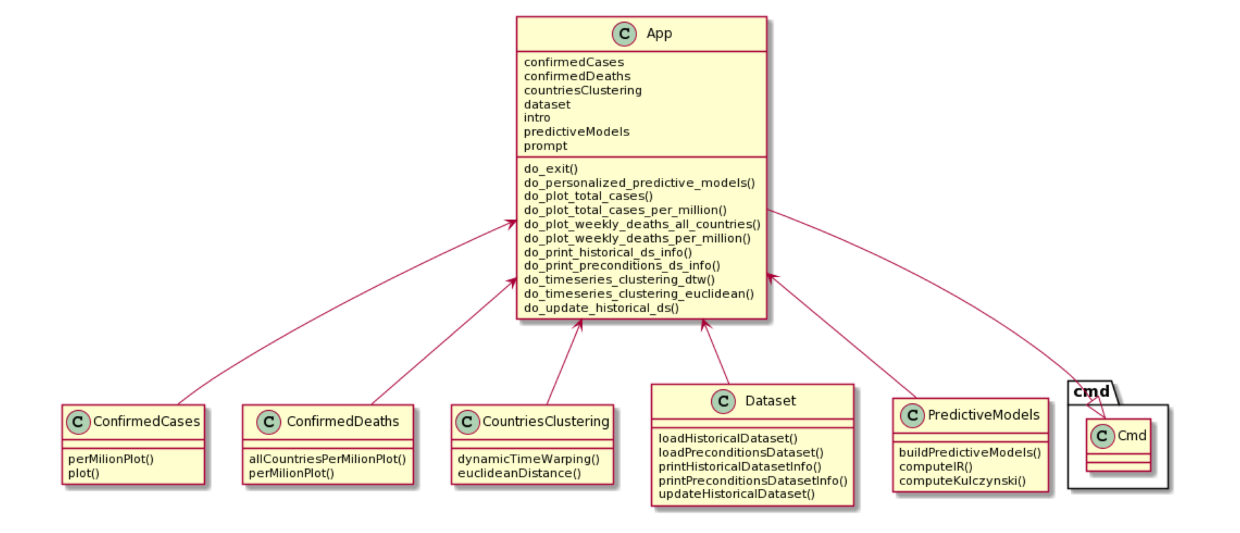
\includegraphics[scale=0.8]{img/class_diagram.pdf}
    \end{center}
    \caption{Python Class Diagram}
\end{figure}
The following is a brief description of each of the classes:
\begin{itemize}
    \item \texttt{App}: application entry point; it implements the command line
    menu logic using an instance of the \texttt{Cmd} Python3 class;
    \item \texttt{Cmd}: this Python3 class provides a simple framework for
    writing line-oriented command interpreters. These are often useful for test
    harnesses, administrative tools, and prototypes that will later be wrapped
    in a more sophisticated interface;
    \item \texttt{ConfirmedCases}: implements all the functions related to
    plotting Confirmed COVID-19 cases;
    \item \texttt{ConfirmedDeaths}: implements all the functions related to
    plotting Confirmed COVID-19 cases;
    \item \texttt{CountriesClustering}: implements all the functions related to
    computing and plotting countries K-means clustering based on COVID-19
    confirmed deaths;
    \item \texttt{Dataset}: implements all the functions related to loading,
    preprocessing, saving and printing the content of the different datasets;
    \item \texttt{PredictiveModels}: implements all the functions related to
    loading, preprocessing, saving and printing the content of the different
    datasets.
\end{itemize}
\subsection{Python Packages}
The following Python3 packages and libraries were used in the development:
\begin{itemize}
    \item \texttt{matplotlib.pyplot}: is a state-based interface to
    \texttt{matplotlib}; it provides a MATLAB-like way of plotting; mainly
    intended for interactive plots and simple cases of programmatic plot
    generation;
    \item \texttt{pandas}: is a fast, powerful, flexible and easy to use open
    source data analysis and manipulation tool, built on top of the Python
    programming language;
    \item \texttt{numpy}: is the fundamental package for scientific computing in
    Python; it is a Python library that provides a multidimensional array
    object, various derived objects (such as masked arrays and matrices), and an
    assortment of routines for fast operations on arrays, including
    mathematical, logical, basic statistical operations, random simulation and
    much more;
    \item \texttt{plotly}: is a high-level, declarative charting library;
    \item \texttt{plotly.graph\_objs}: the figures created, manipulated and
    rendered by the \texttt{plotly} Python library are represented by tree-like
    data structures which are automatically serialized to JSON for rendering by
    the \texttt{Plotly.js} JavaScript library.
    \item \texttt{sklearn}: Scikit-learn (formerly \texttt{scikits.learn}) is a
    free software machine learning library for the Python programming language;
    \item \texttt{tslearn}: is a Python package that provides machine learning
    tools for the analysis of time series;
    \item \texttt{tslearn.utils}: is a which module includes various time
    series conversion utilities;
    \item \texttt{tslearn.clustering}: K-means clustering for time-series data;
    \item \texttt{mlxtend}: Mlxtend (machine learning extensions) is a Python
    library of useful tools for the day-to-day data science tasks;
    \item \texttt{mlxtend.frequent\_patterns}: this module contains the Apriori
    and FPGrowth algorithm implementations.
\end{itemize}
\subsection{Kulczynski measure and Imbalance Ratio}
The \texttt{frequent\_patterns} module of the \texttt{mlxtend} Python package
used to mine the association rules, provides the following scoring metrics:
"antecedent support", "consequent support", "support", "confidence", "lift",
"leverage" and "conviction".\\
\\
The Kulczynski measure was computed using the provided metrics according to the
following reasoning:
$$
    Kulc(A, B) = \frac{1}{2}\left(P(A|B) + P(B|A)\right) =
$$
\vspace*{0.1cm}
$$
    = \frac{1}{2}\left(\frac{support(B \cup A)}{support(B)} +
    \frac{support(A \cup B)}{support(A)}\right) =
$$
\vspace*{0.1cm}
$$
    = \frac{1}{2}\left(\frac{"support"}{"consequent\ support"} +
    \frac{"support"}{"antecedent\ support"}\right).
$$
\\
\\
The Imbalance Ratio was computed using the provided metrics according to the
following reasoning:
$$
    IR(A, B) = \frac{|support(A) - support(B)|}{support(A) - support(B)
    + support(A \cup B)} =
$$
\vspace*{0.1cm}
$$
    = \frac{|"antecedent\ support" - "consequent\ support"|}
    {"antecedent\ support" - "consequent\ support" + "support"}.
$$
%-------------------------------------------------------------------------------
% Bibliography
%-------------------------------------------------------------------------------
\newpage
\printbibliography

\end{document}
